% $Header: /home/vedranm/bitbucket/beamer/solutions/generic-talks/generic-ornate-15min-45min.en.tex,v 90e850259b8b 2007/01/28 20:48:30 tantau $

\documentclass{beamer}

% This file is a solution template for:

% - Giving a talk on some subject.
% - The talk is between 15min and 45min long.
% - Style is ornate.



% Copyright 2004 by Till Tantau <tantau@users.sourceforge.net>.
%
% In principle, this file can be redistributed and/or modified under
% the terms of the GNU Public License, version 2.
%
% However, this file is supposed to be a template to be modified
% for your own needs. For this reason, if you use this file as a
% template and not specifically distribute it as part of a another
% package/program, I grant the extra permission to freely copy and
% modify this file as you see fit and even to delete this copyright
% notice.


\mode<presentation>
{
  \usetheme{Warsaw}
  % or ...

  \setbeamercovered{transparent}
  % or whatever (possibly just delete it)
}

      \theoremstyle{theorem}
      \newtheorem{proposition}[theorem]{Proposition}
      \theoremstyle{definition}
      \newtheorem{game}[theorem]{Game}
      \newtheorem{question}[theorem]{Question}

\usepackage[english]{babel}
% or whatever

\usepackage[latin1]{inputenc}
% or whatever

\usepackage{times}
\usepackage[T1]{fontenc}
% Or whatever. Note that the encoding and the font should match. If T1
% does not look nice, try deleting the line with the fontenc.


\usepackage{marvosym} % For \Smiley
\usepackage{verbatim} % for \verbatiminput

\title
{Games and Mathematics}

\subtitle
{Huntingdon College} % (optional)

\author%[Author, Another] % (optional, use only with lots of authors)
{Steven~Clontz~\\http://stevenclontz.com}%\inst{1} \and S.~Another\inst{2}}
% - Use the \inst{?} command only if the authors have different
%   affiliation.

\institute[Auburn University] % (optional, but mostly needed)
{
  %\inst{1}%
  Department of Mathematics and Statistics\\
  Auburn University}
  %\and
  %\inst{2}%
  %Department of Theoretical Philosophy\\
  %University of Elsewhere}
% - Use the \inst command only if there are several affiliations.
% - Keep it simple, no one is interested in your street address.

\date[14-06-23] % (optional)
{June 23, 2014}


% If you have a file called "university-logo-filename.xxx", where xxx
% is a graphic format that can be processed by latex or pdflatex,
% resp., then you can add a logo as follows:

 % \pgfdeclareimage[height=1cm]{university-logo}{auburn_logo.png}
 % \logo{\pgfuseimage{university-logo}}



% Delete this, if you do not want the table of contents to pop up at
% the beginning of each subsection:
%\AtBeginSubsection[]
%{
%  \begin{frame}<beamer>{Outline}
%    \tableofcontents[currentsection,currentsubsection]
%  \end{frame}
%}


% If you wish to uncover everything in a step-wise fashion, uncomment
% the following command:

%\beamerdefaultoverlayspecification{<+->}

% My game notational definitions
\newcommand{\win}{\uparrow}
\newcommand{\prewin}{\uparrow_{\text{pre}}}
\newcommand{\markwin}{\uparrow_{\text{mark}}}
\newcommand{\tactwin}{\uparrow_{\text{tact}}}
\newcommand{\ktactwin}[1]{\uparrow_{#1\text{-tact}}}
\newcommand{\kmarkwin}[1]{\uparrow_{#1\text{-mark}}}
\newcommand{\codewin}{\uparrow_{\text{code}}}
\newcommand{\limitwin}{\uparrow_{\text{limit}}}
\newcommand{\oneptcomp}[1]{#1^*}
\newcommand{\oneptlind}[1]{#1^\dagger}
\newcommand{\congame}[2]{Con_{\pl O\pl P}(#1,#2)}
\newcommand{\clusgame}[2]{Clus_{\pl O\pl P}(#1,#2)}
\newcommand{\lfkpgame}[1]{LF_{\pl K\pl P}(#1)}
\newcommand{\lfklgame}[1]{LF_{\pl K\pl L}(#1)}
\newcommand{\pfgame}[1]{PF_{\pl F\pl C}(#1)}
\newcommand{\mengame}[1]{Cov_{\pl C\pl F}(#1)}
\newcommand{\rothgame}[1]{Cov_{\pl C\pl S}(#1)}
\newcommand{\altrothgame}[1]{Cov_{\pl P\pl O}(#1)}
\newcommand{\fillgame}[1]{Fill^{\subseteq}_{\pl M\pl N}(#1)}
\newcommand{\sfillgame}[1]{Fill^{\subsetneq}_{\pl M\pl N}(#1)}
\newcommand{\kfillgame}[1]{Fill^{\subseteq}_{\pl C\pl F}(#1)}
\newcommand{\ksfillgame}[1]{Fill^{\subsetneq}_{\pl C\pl F}(#1)}
\newcommand{\recallgame}[2]{Rec^{#1}_{\pl F\pl S}(#2)}
\newcommand{\sigmaprodr}[1]{\Sigma\mathbb{R}^{#1}}
\newcommand{\sigmaprodtwo}[1]{\Sigma2^{#1}}
\newcommand{\concat}{^\frown}
\newcommand{\rest}{\restriction}
\newcommand{\cl}[1]{\overline{#1}}
\newcommand{\pow}[1]{\mc{P}(#1)}
\newcommand{\<}{\langle}
\renewcommand{\>}{\rangle}
\newcommand{\al}[1]{{#1}^*}
\newcommand{\mc}[1]{\mathcal{#1}}
\newcommand{\po}{\mathbb{P}}
\newcommand{\pok}{\po_\kappa}
\newcommand{\Lim}{\mathrm{Lim}}
\newcommand{\Suc}{\mathrm{Suc}}
\newcommand{\ds}{\displaystyle}
\newcommand{\alcomp}{\al\parallel}
\newcommand{\rank}{\textrm{rank}}
\newcommand{\dom}{\textrm{dom}}
\newcommand{\scish}{almost-$\sigma$-(relatively compact)}

\usepackage{mathrsfs}
\newcommand{\pl}[1]{\mathscr{#1}}

\newcommand{\vpause}{\pause\vspace{1em}}

\newcommand{\term}[1]{\textbf{#1}}




\begin{document}
\renewcommand{\pause}{}

\begin{frame}
  \titlepage
\end{frame}

% \begin{frame}{Table of Contents}
%   \tableofcontents
%   % You might wish to add the option [pausesections]
% \end{frame}

\section{Introduction}

\subsection{Abstract}

\begin{frame}{Abstract}%{Subtitles are optional.}
    \small
    Two player games of perfect information such as chess and checkers have
    been played for centuries. Such games can be analyzed using tools from
    the field of game theory.

    \vpause

    We will define two simple games: Takeaway and Nim.
    Using game theory, we will show how to create a \term{winning strategy}
    for one of the players in each game.

    \vpause

    Also, we will show how \textit{any} game can be analyzed in order
    to produce a winning strategy (given enough computational power).
\end{frame}

\subsection{What's Game Theory?}

\begin{frame}{About game theory}
  Game theory is a broad subject, but in any context, it typically involves the
  mathematics of decision making.

  \vpause

  Economists use game theory to study \term{two-player simultaneous}
  games. Suppose two companies have to set a price on competiting products.
  The demand for each product depends on the decisions made by both companies.
  The \term{Prisoner's Delimma} is another example of this type of game.

  \vpause

  Another example would be \term{games of chance} like Solitaire or Yahtzee.
  One or more players use dice rolls or a shuffled deck of cards to play such
  games, and have to use probability to make decisions based upon future rolls
  of the dice or face-down cards.
\end{frame}

\begin{frame}{Two-player Sequential Games}
  We'll be talking about \term{two-player sequential} games today. These are
  games of \term{perfect information}: the players take turns with full
  knowledge of the history of their opponent's moves.

  \vspace{1em}

  \centerline{
    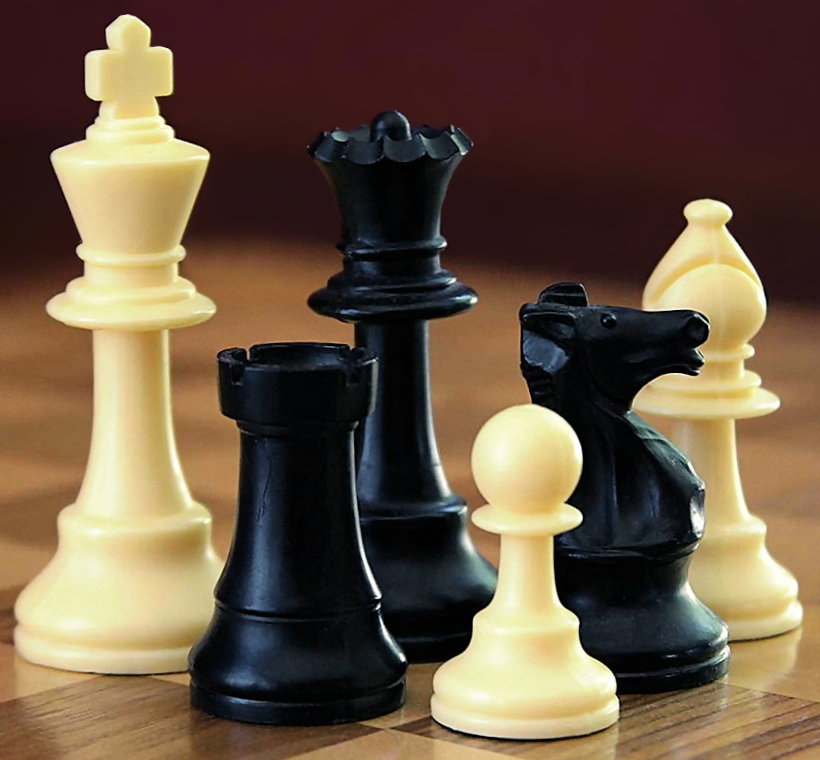
\includegraphics[height=1.5in]{chessPieces.jpg}
    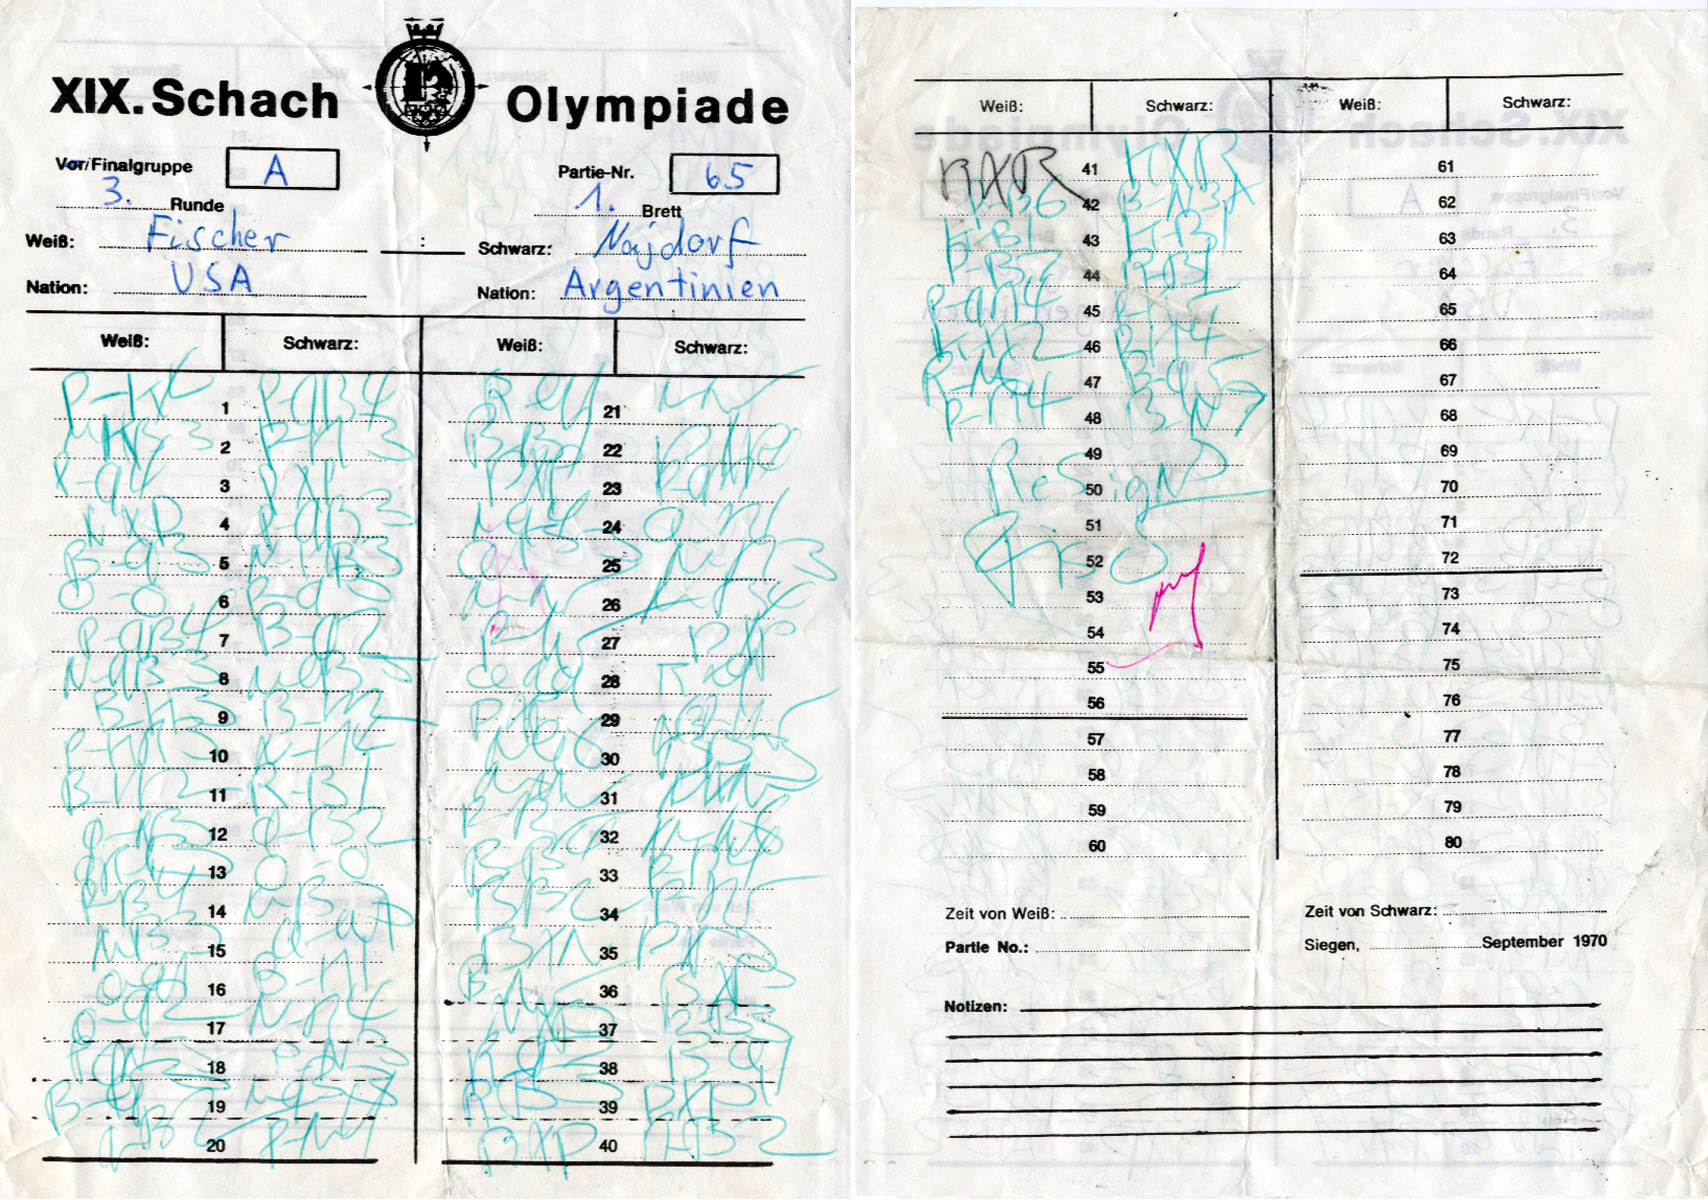
\includegraphics[height=1.5in]{chessNotation.jpg}
  }
\end{frame}

\section{A Couple of Basic Games}

\begin{frame}{Coin games}
  The two games we'll talk about are \term{coin games}, because they can be
  played with whatever loose change you have in your pocket.

  \centerline{
    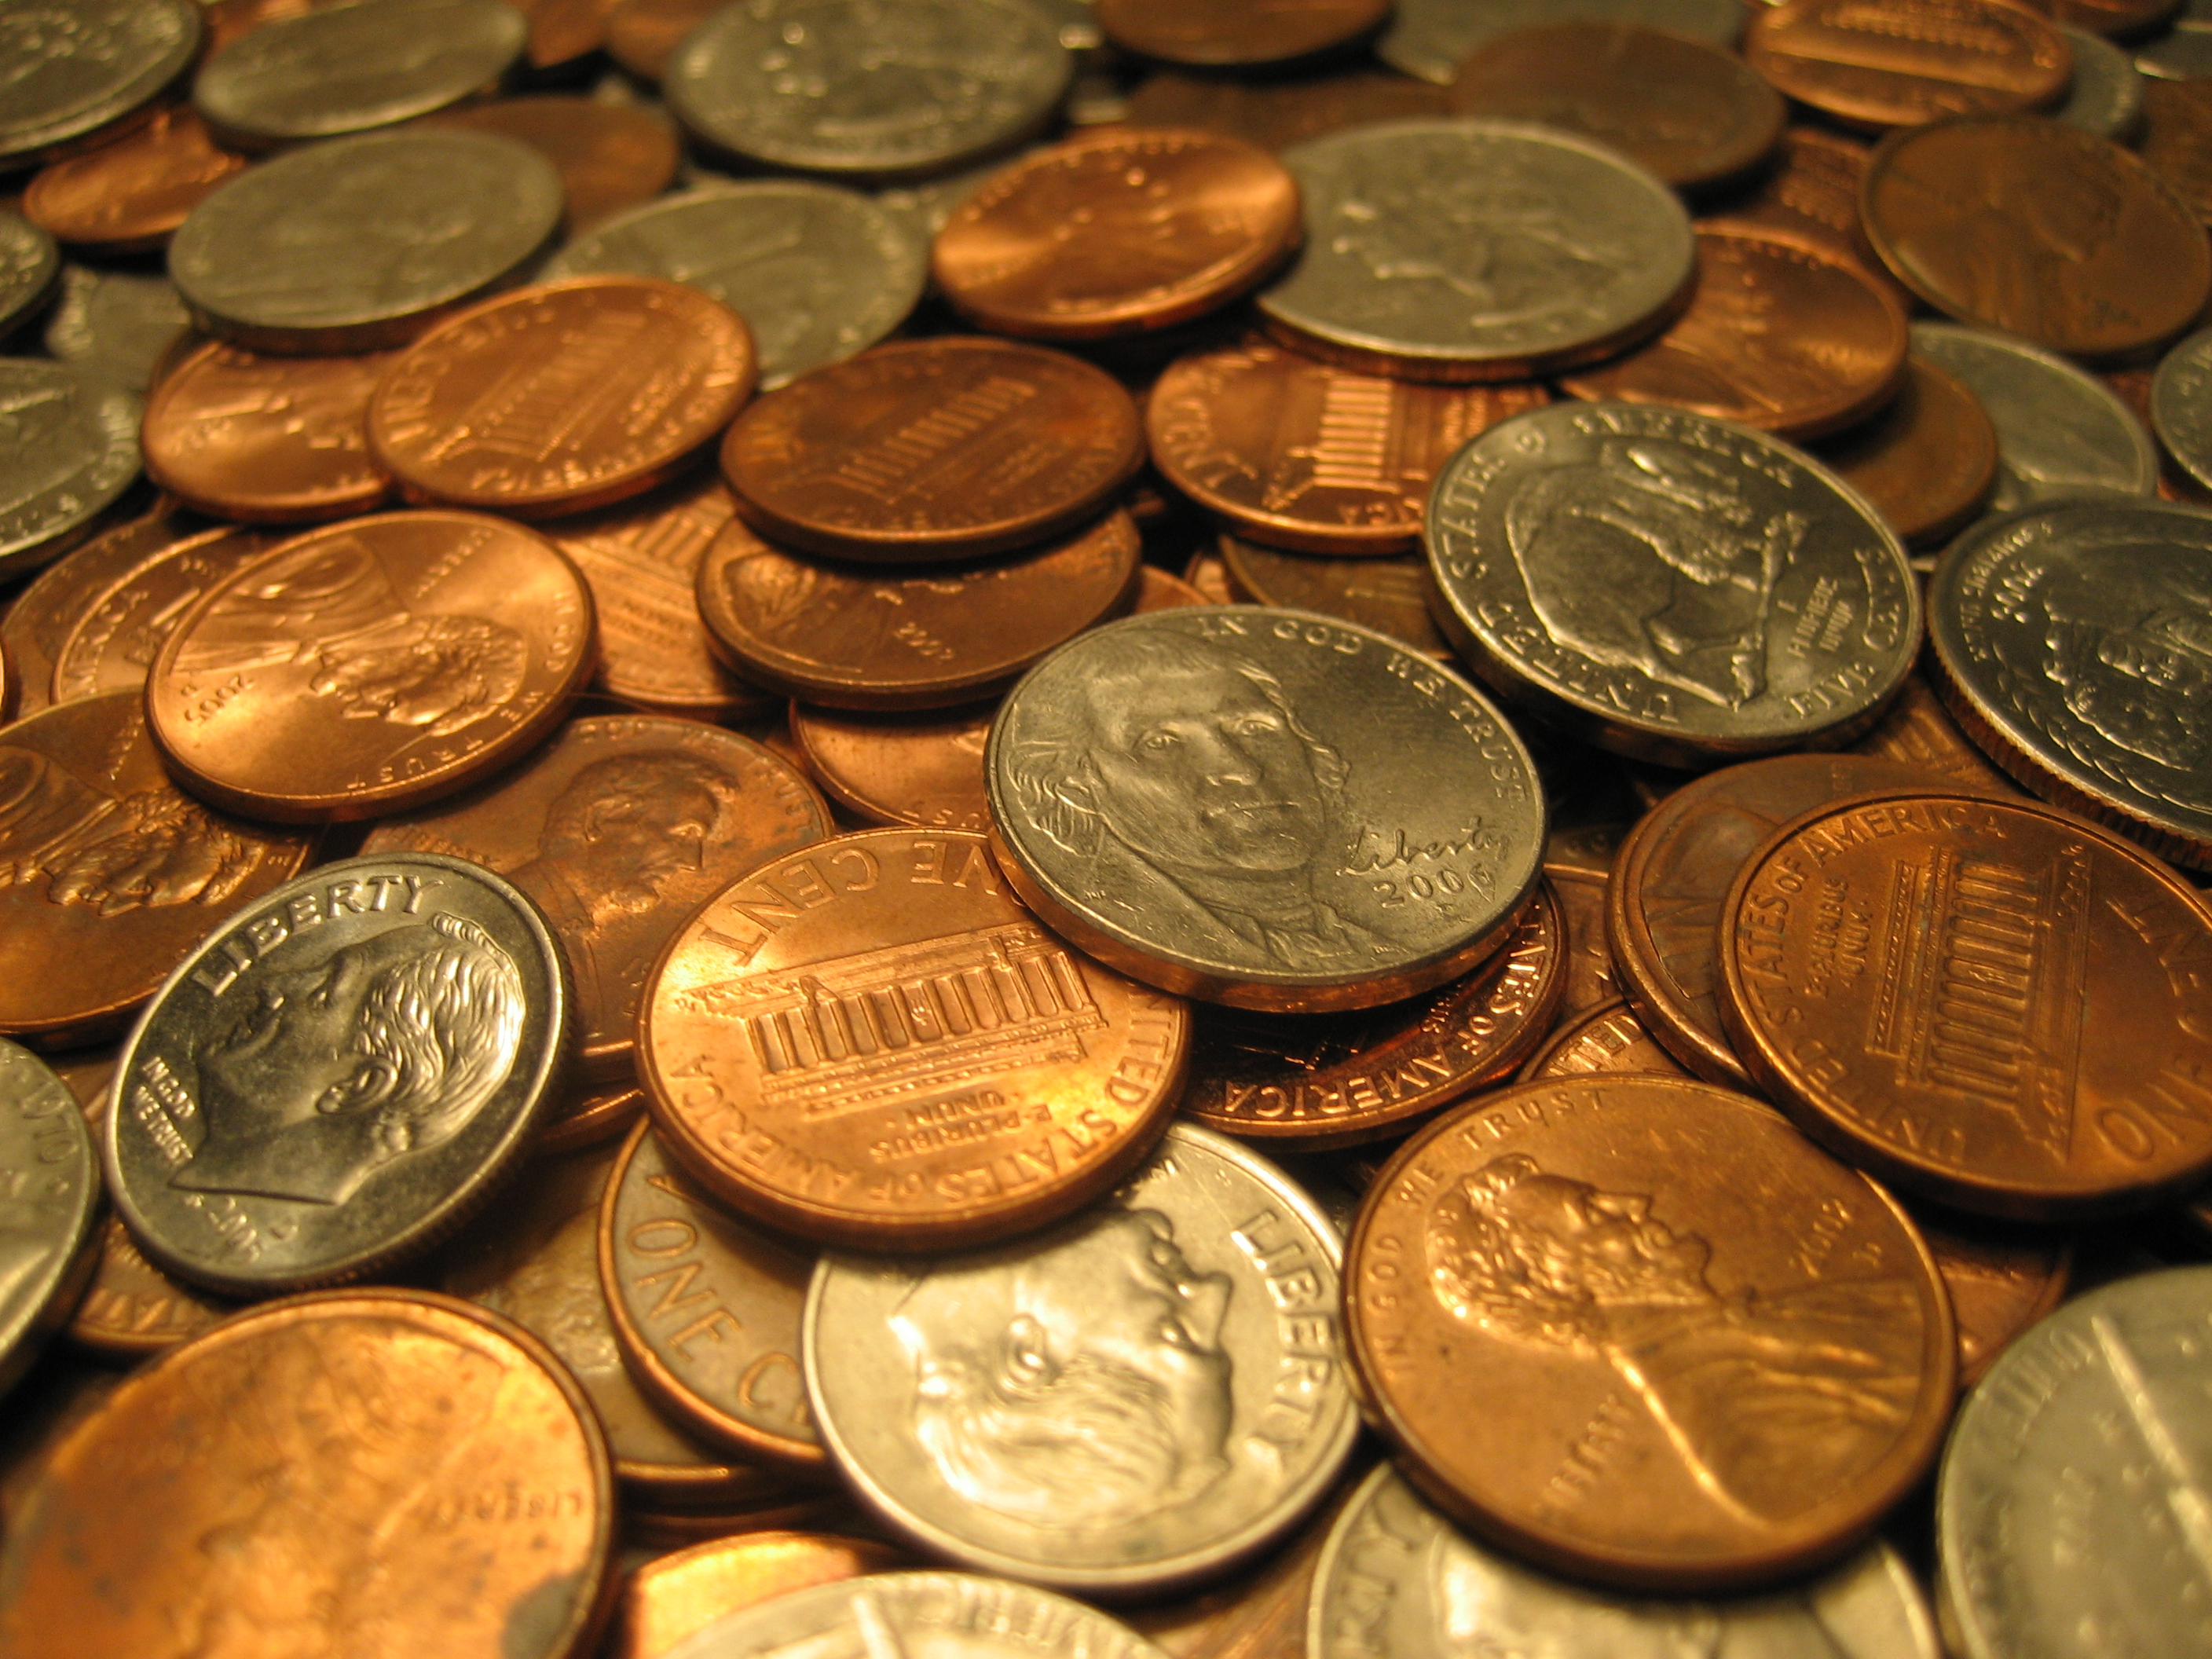
\includegraphics[height=2in]{coins.jpg}
  }
\end{frame}

\subsection{Takeaway}

\begin{frame}{Takeaway}
  In \term{Takeaway}, the Players $\pl A$, $\pl B$ take turns removing $1$,
  $2$, or $3$ coins from the table. The player who
  removes the last coin wins.

  \vspace{1em}

  \centerline{
    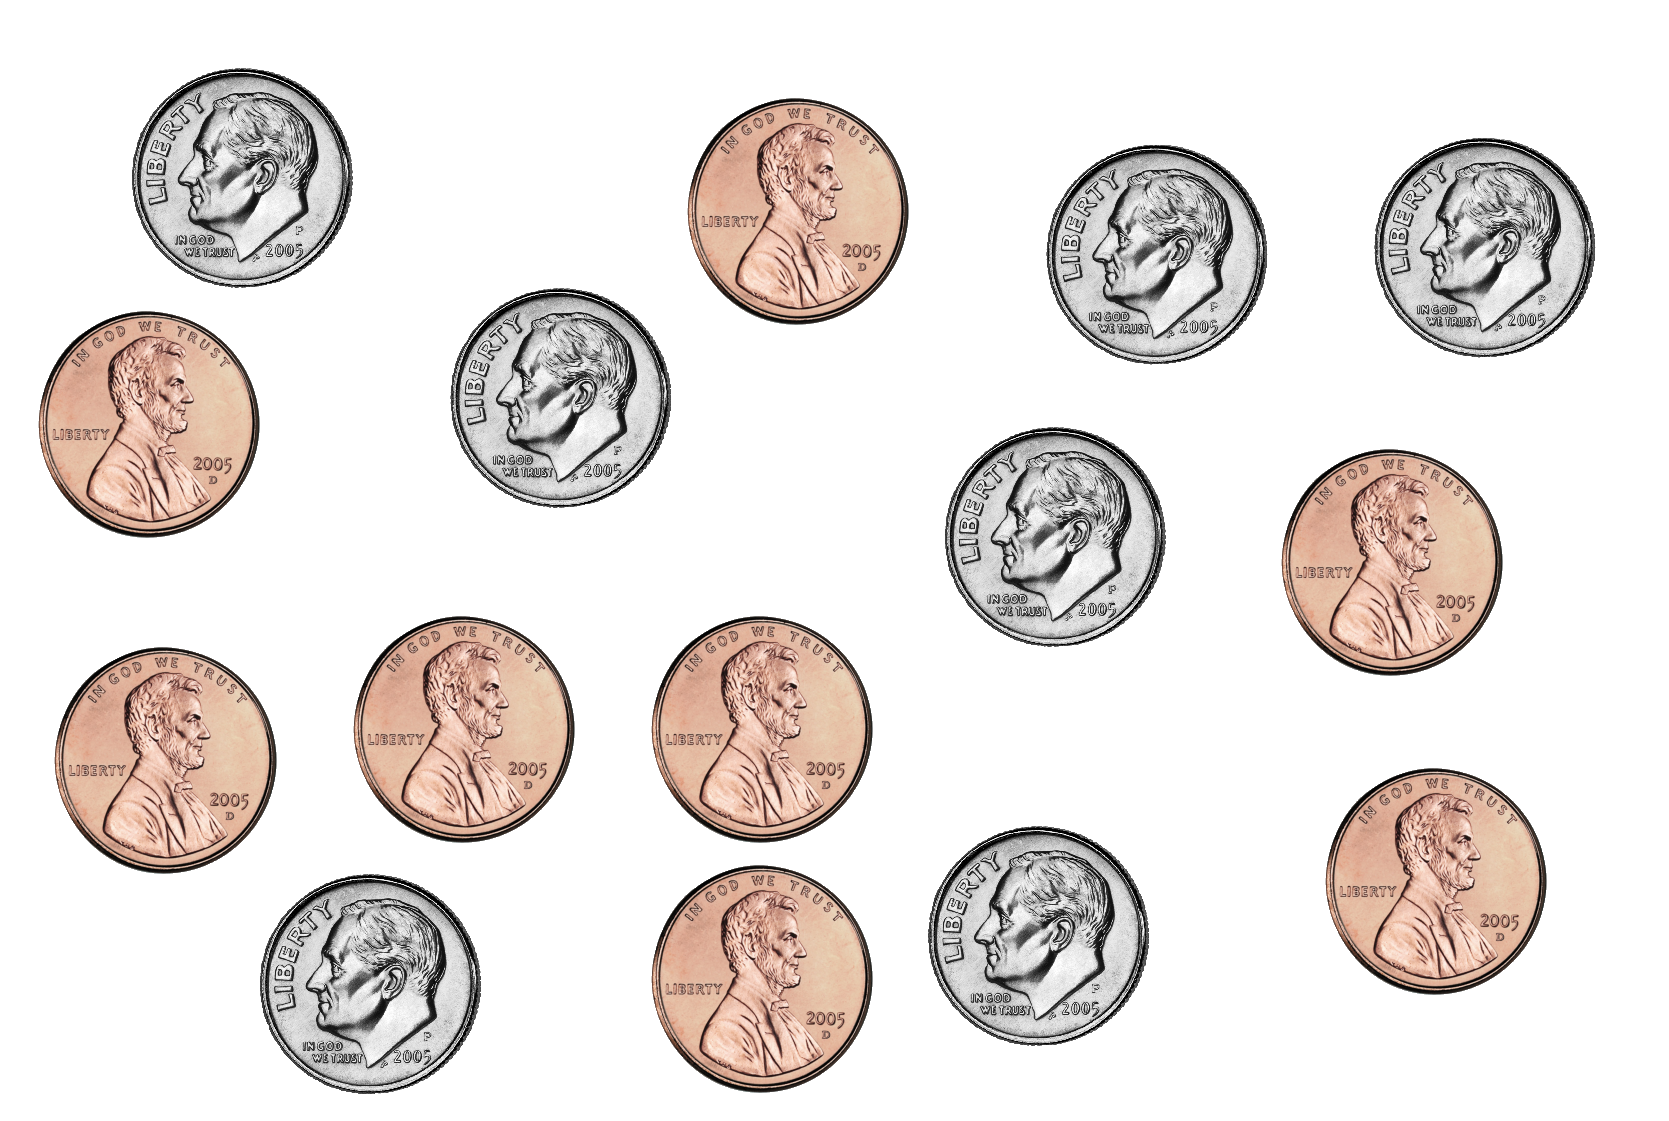
\includegraphics[height=1.7in]{takeawayCoins/15.pdf}
  }
\end{frame}

\begin{frame}
  Round 1a: Player $\pl A$ takes away 3 coins, leaving 12.

  \centerline{
    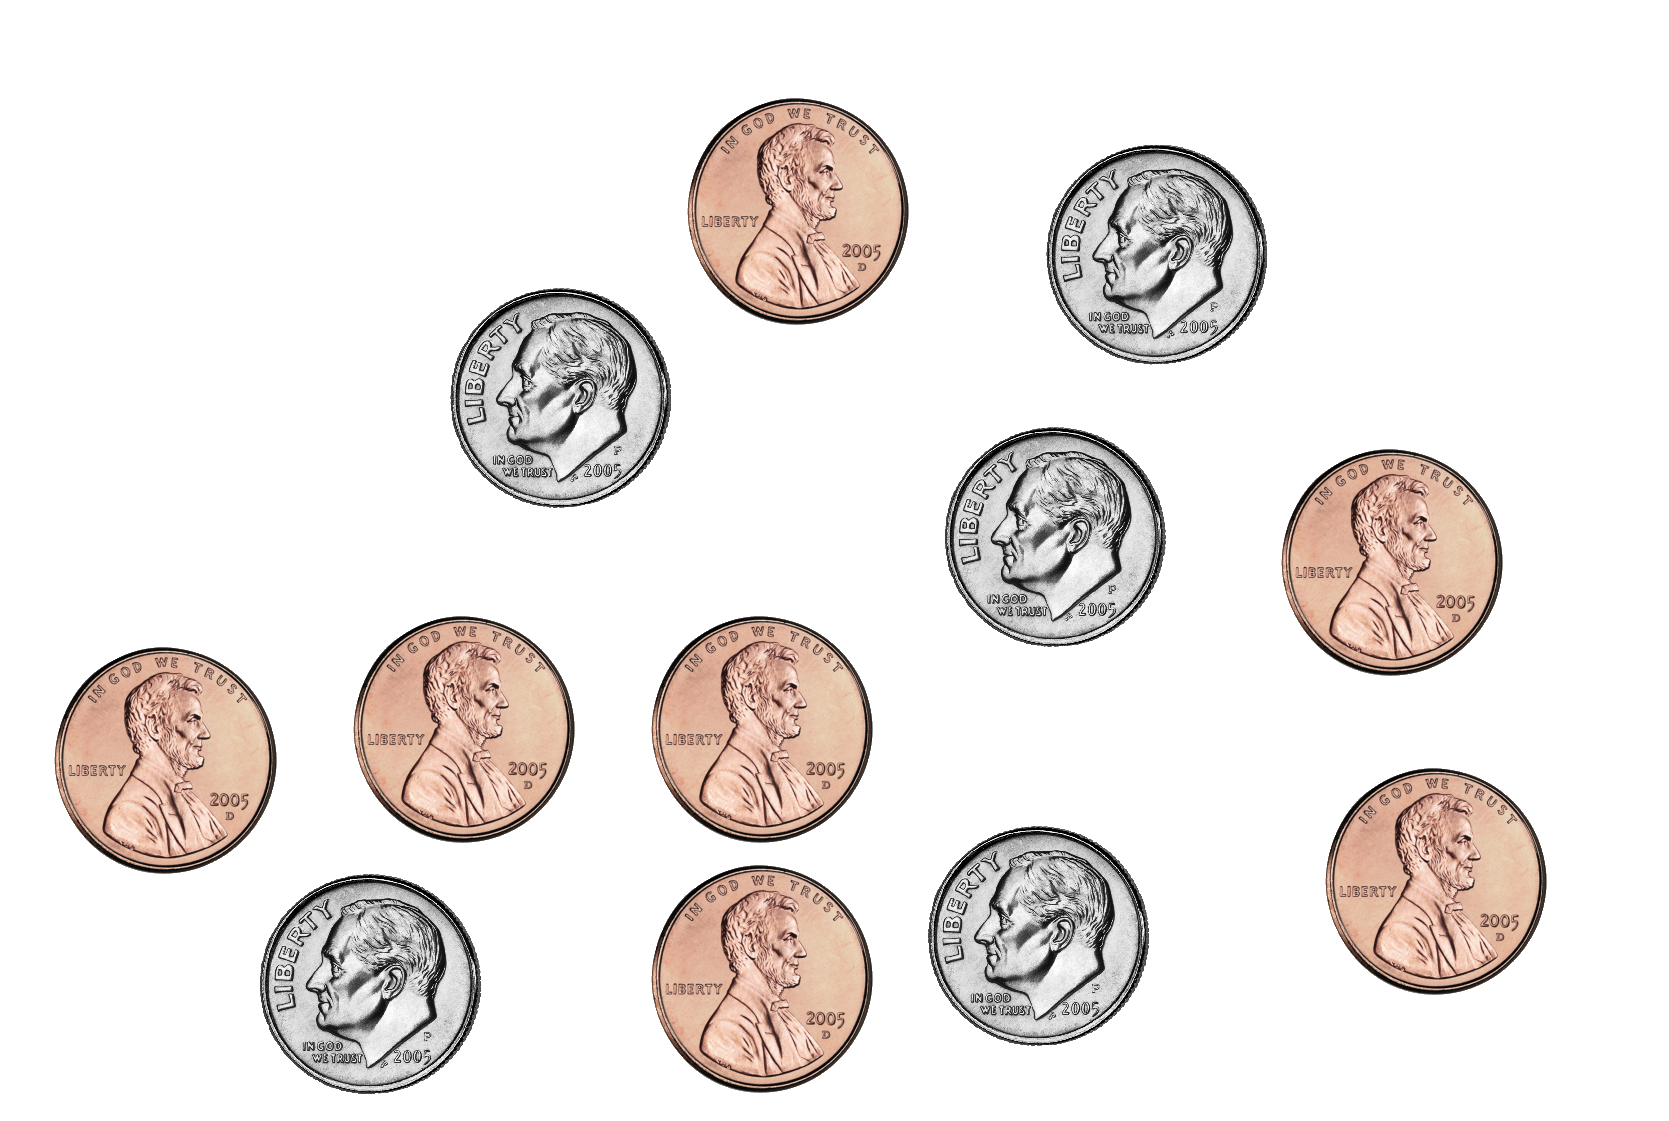
\includegraphics[height=1.7in]{takeawayCoins/12.pdf}
  }
\end{frame}

\begin{frame}
  Round 1b: Player $\pl B$ takes away 2 coins, leaving 10.

  \centerline{
    
\includegraphics[height=1.7in]{takeawayCoins/10.pdf}
  }
\end{frame}

\begin{frame}
  Round 2a: Player $\pl A$ takes away 1 coin, leaving 9.

  \centerline{
    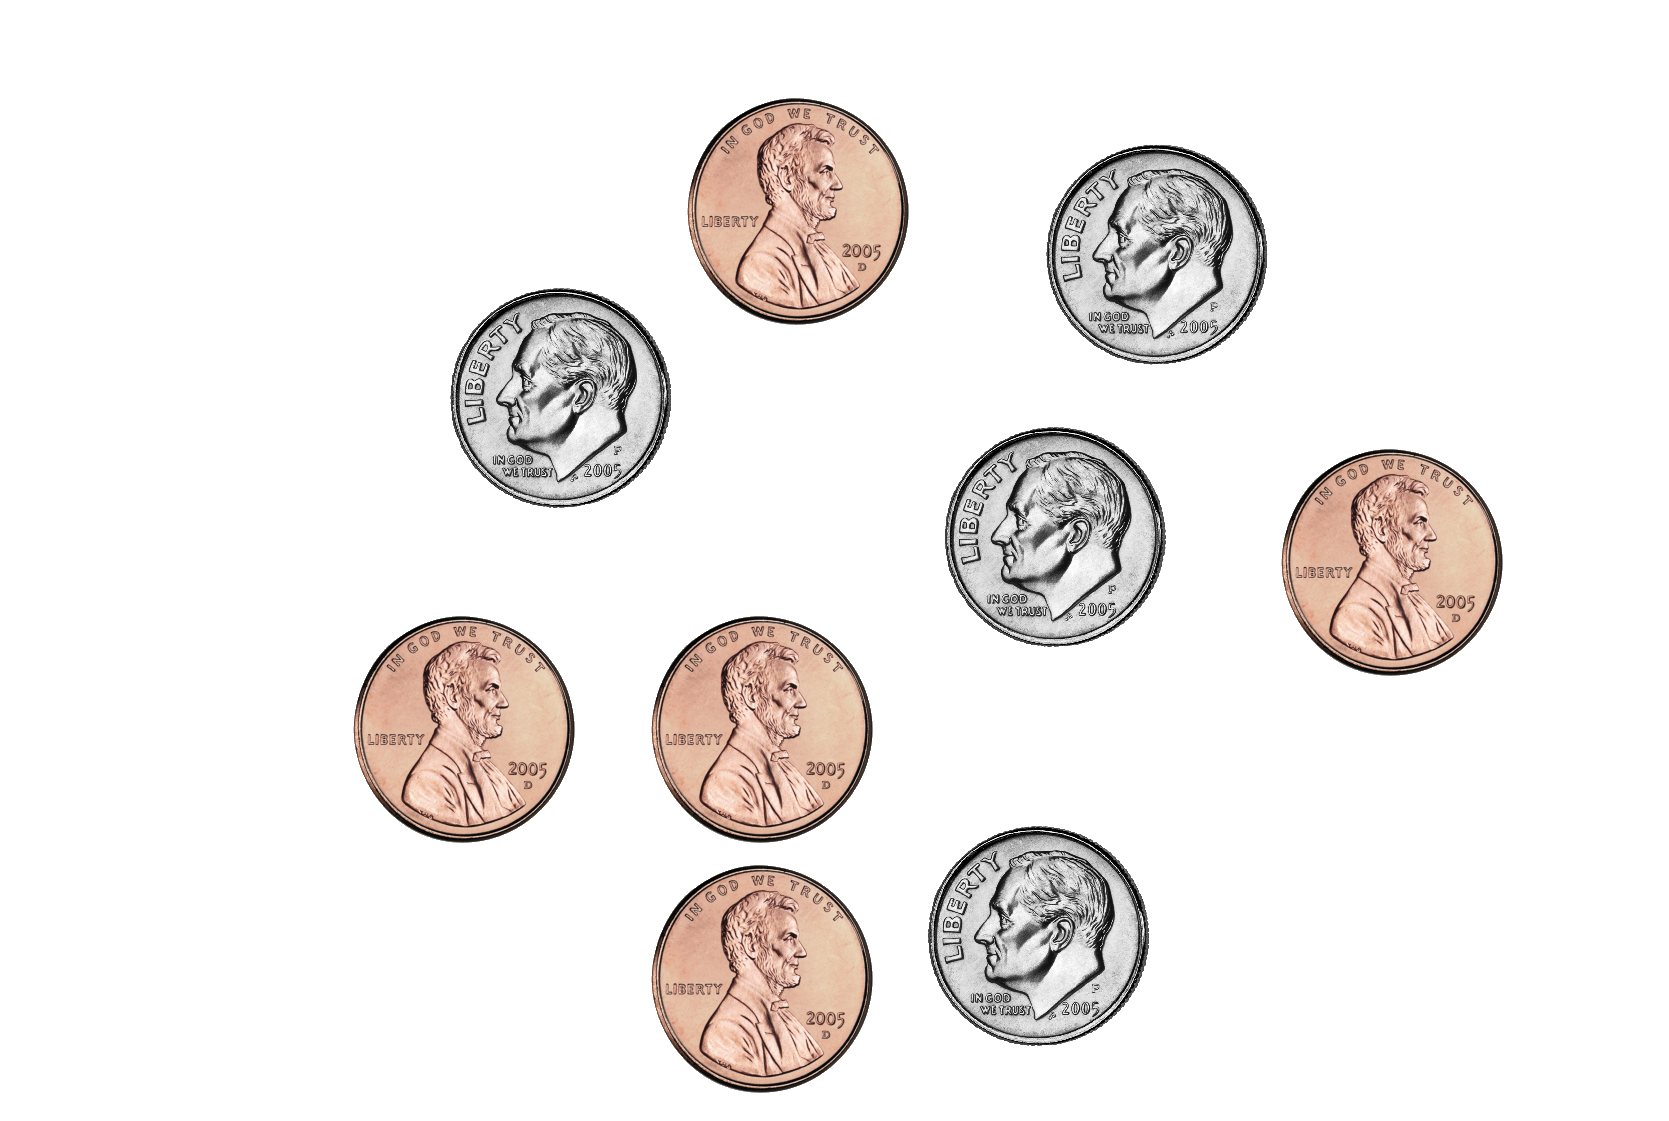
\includegraphics[height=1.7in]{takeawayCoins/09.pdf}
  }
\end{frame}

\begin{frame}
  Round 2b: Player $\pl B$ takes away 2 coins, leaving 7.

  \centerline{
    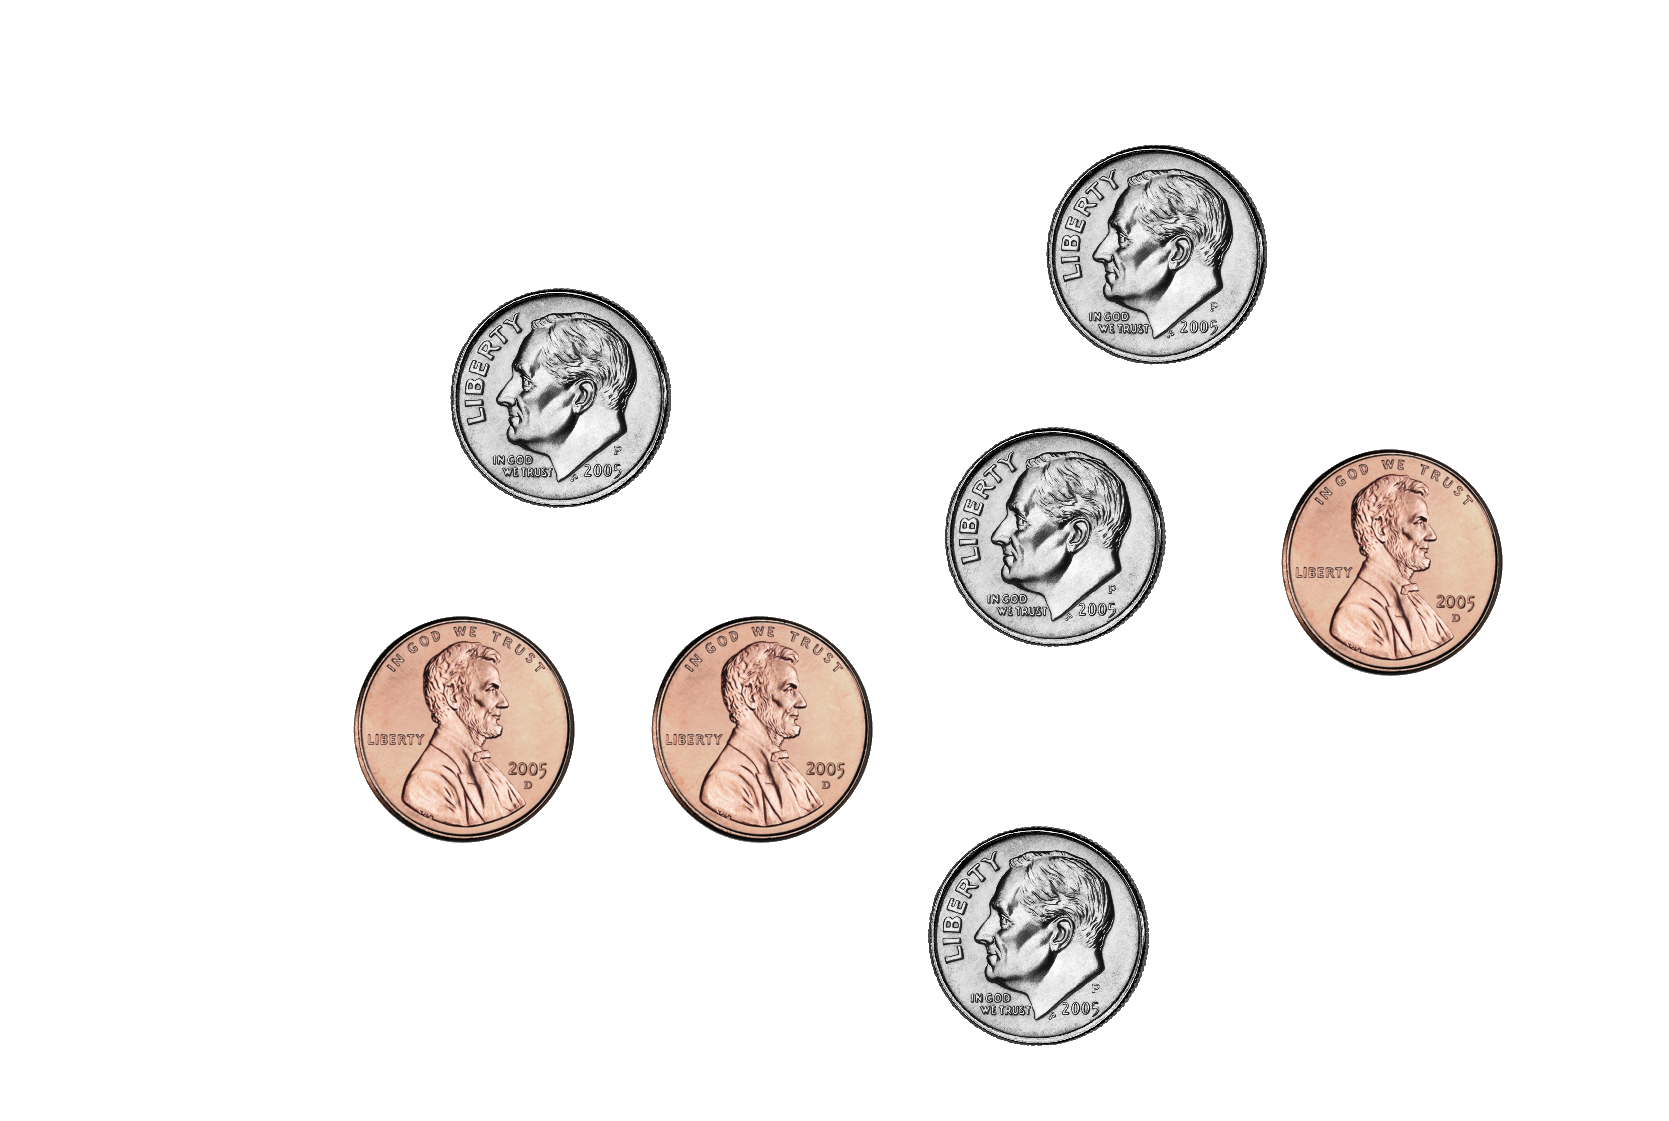
\includegraphics[height=1.7in]{takeawayCoins/07.pdf}
  }
\end{frame}

\begin{frame}
  Round 3a: Player $\pl A$ takes away 1 coin, leaving 6.

  \centerline{
    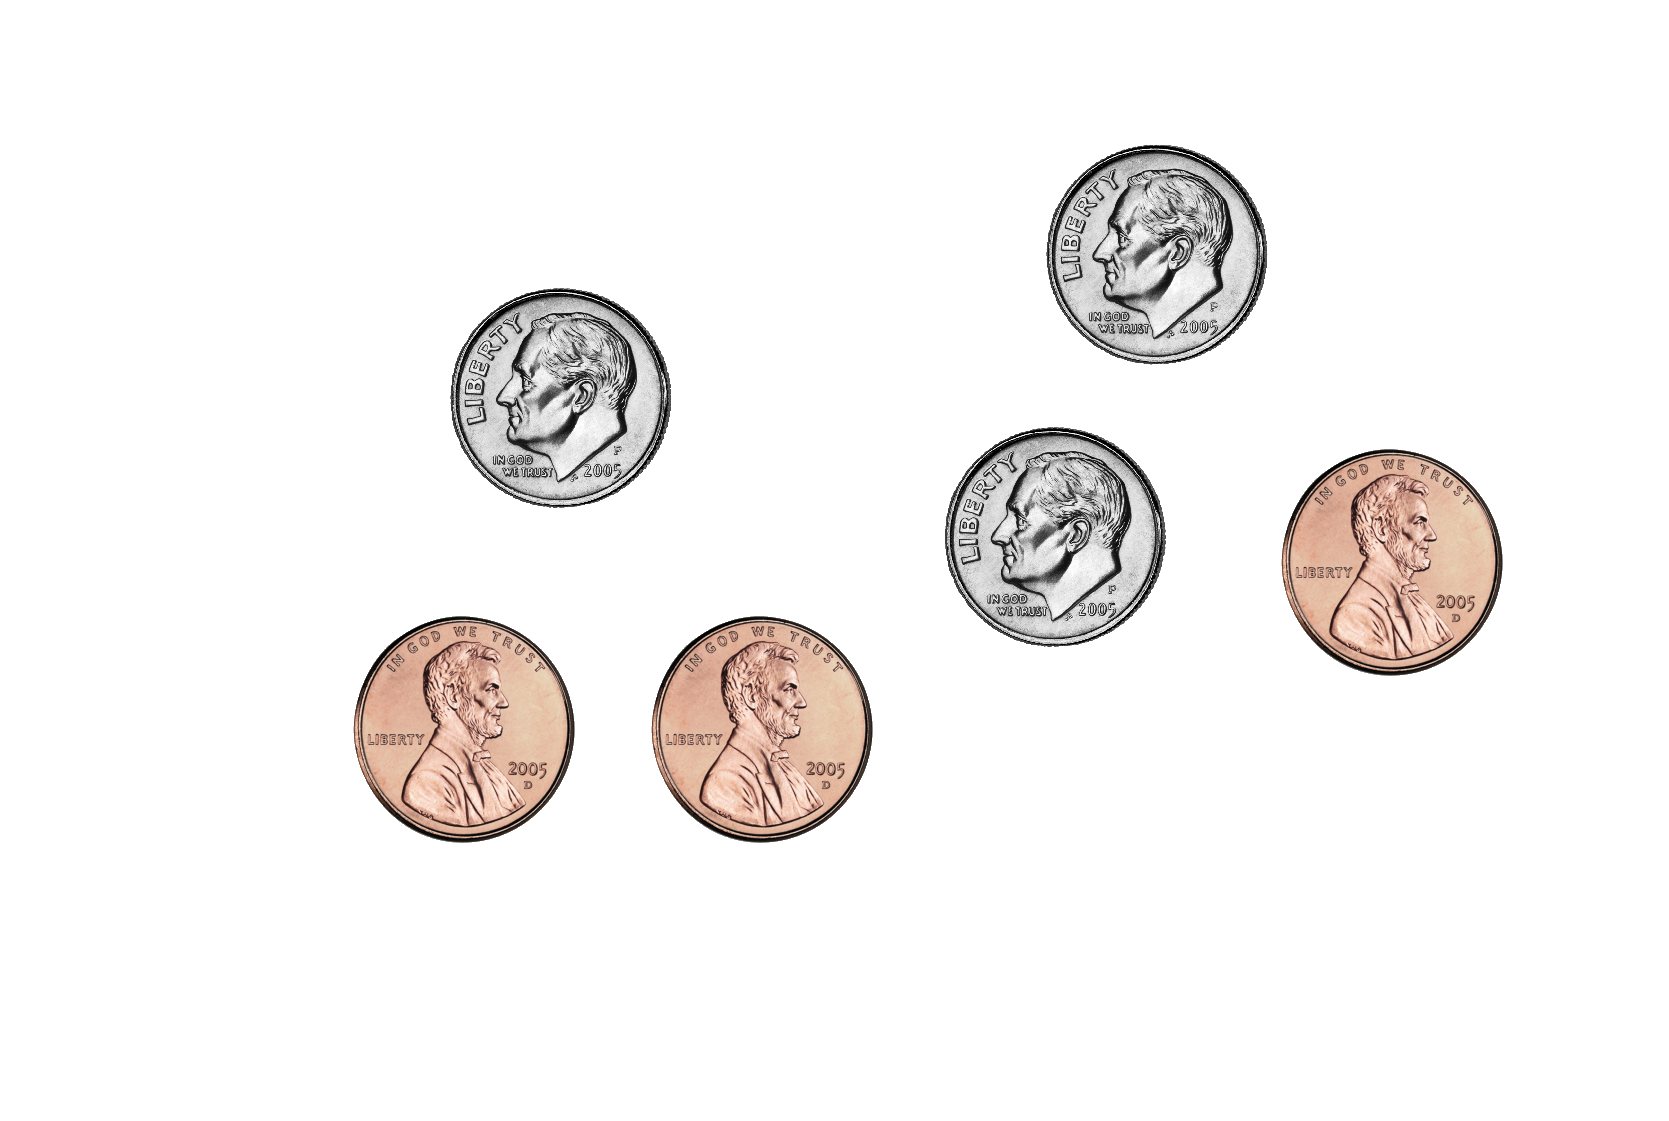
\includegraphics[height=1.7in]{takeawayCoins/06.pdf}
  }
\end{frame}

\begin{frame}
  Round 3b: Player $\pl B$ takes away 2 coins, leaving 4.

  \centerline{
    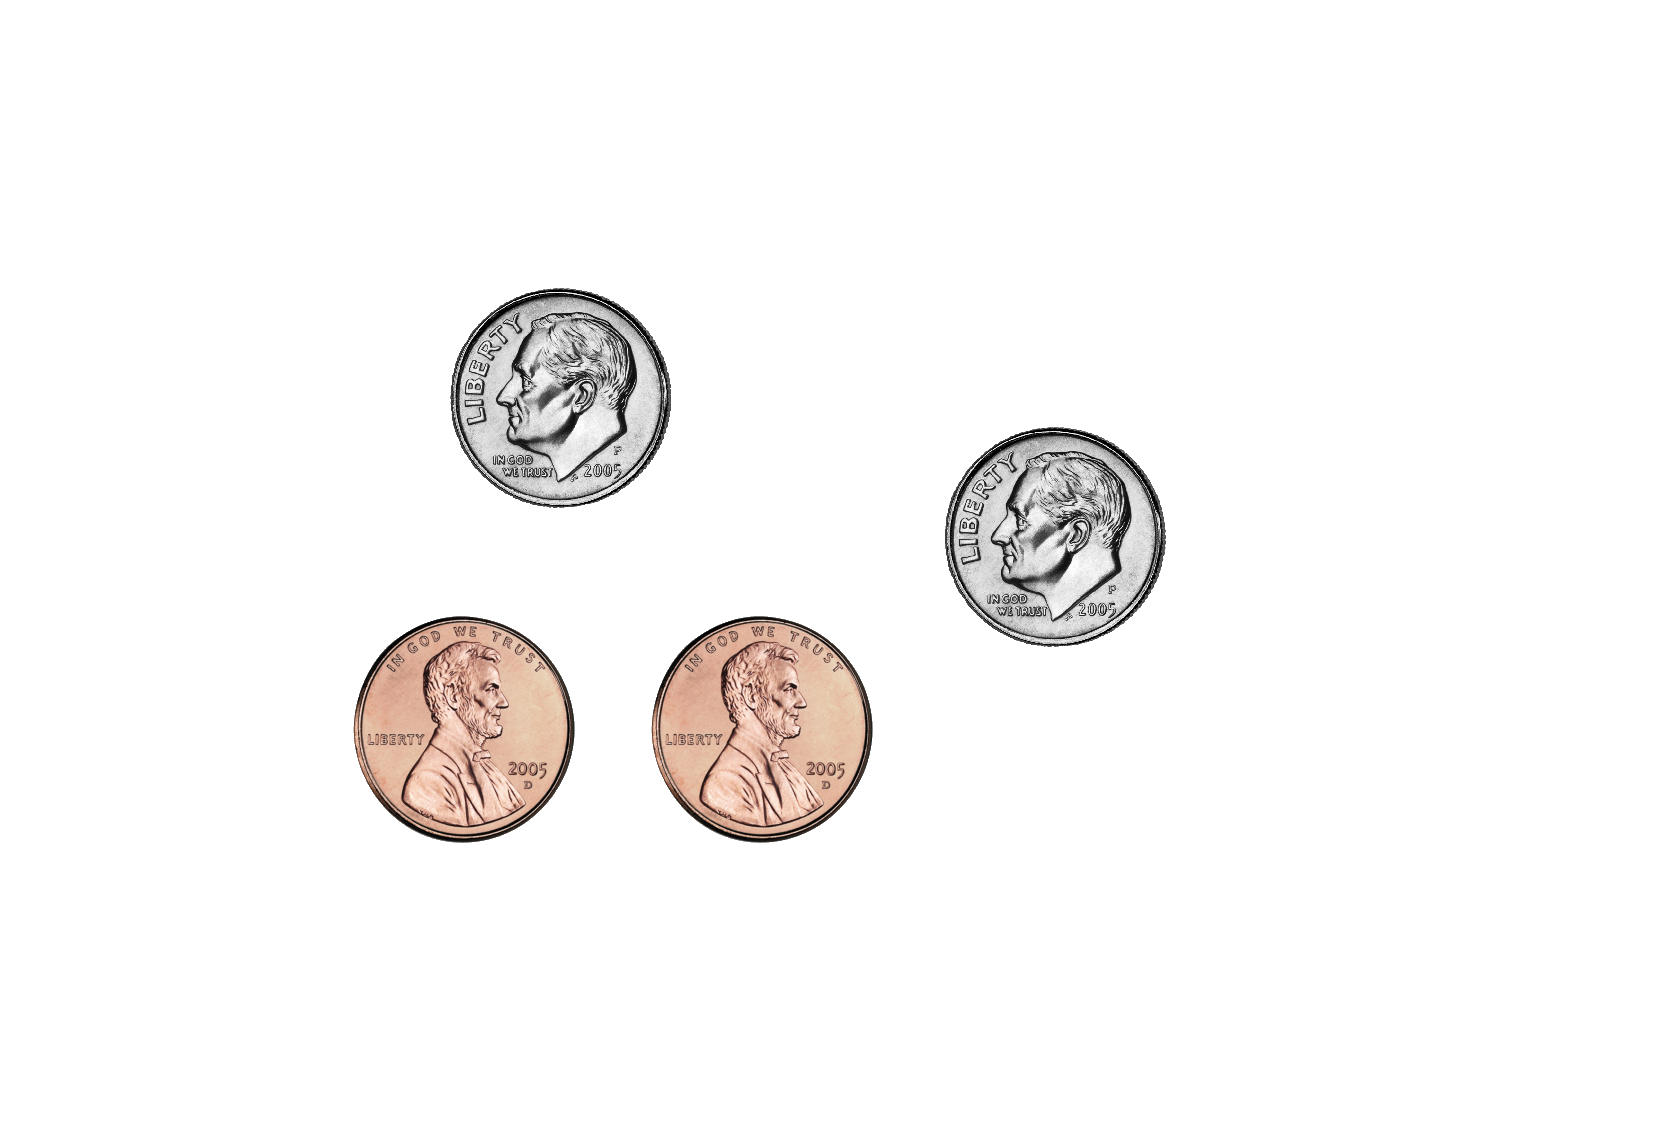
\includegraphics[height=1.7in]{takeawayCoins/04.pdf}
  }
\end{frame}

\begin{frame}
  Round 4a: Player $\pl A$ takes away 1 coin, leaving 3.

  \centerline{
    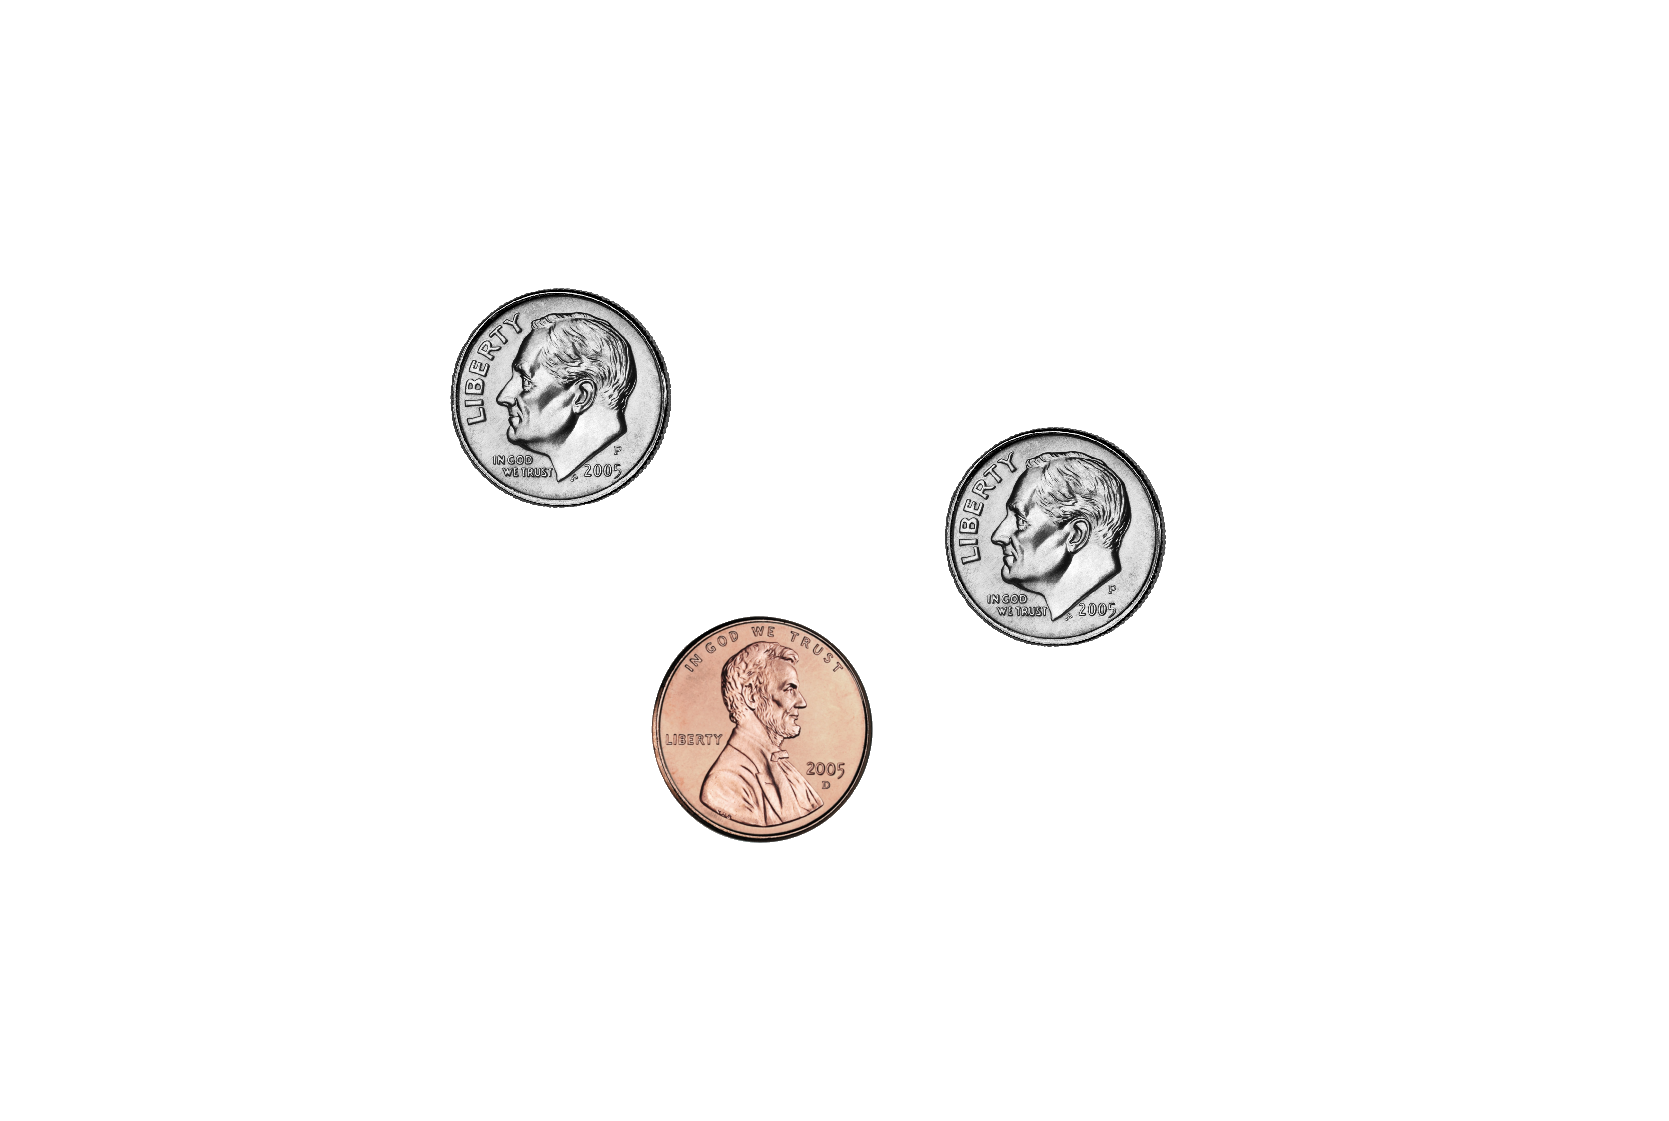
\includegraphics[height=1.7in]{takeawayCoins/03.pdf}
  }
\end{frame}

\begin{frame}
  Round 4b: Player $\pl B$ takes away the last 3 coins, and wins!

  \centerline{
    
\includegraphics[height=1.7in]{takeawayCoins/00.pdf}
  }
\end{frame}

\begin{frame}{A winning strategy}
  When studying sequential games, we often want to find what's called
  a \term{winning strategy}. Such a strategy should guarantee that the player
  following it cannot lose the game.

  \vpause

  I claim that when Takeaway starts with $12$ coins, then Player $\pl B$ has
  a winning strategy.

  \centerline{
    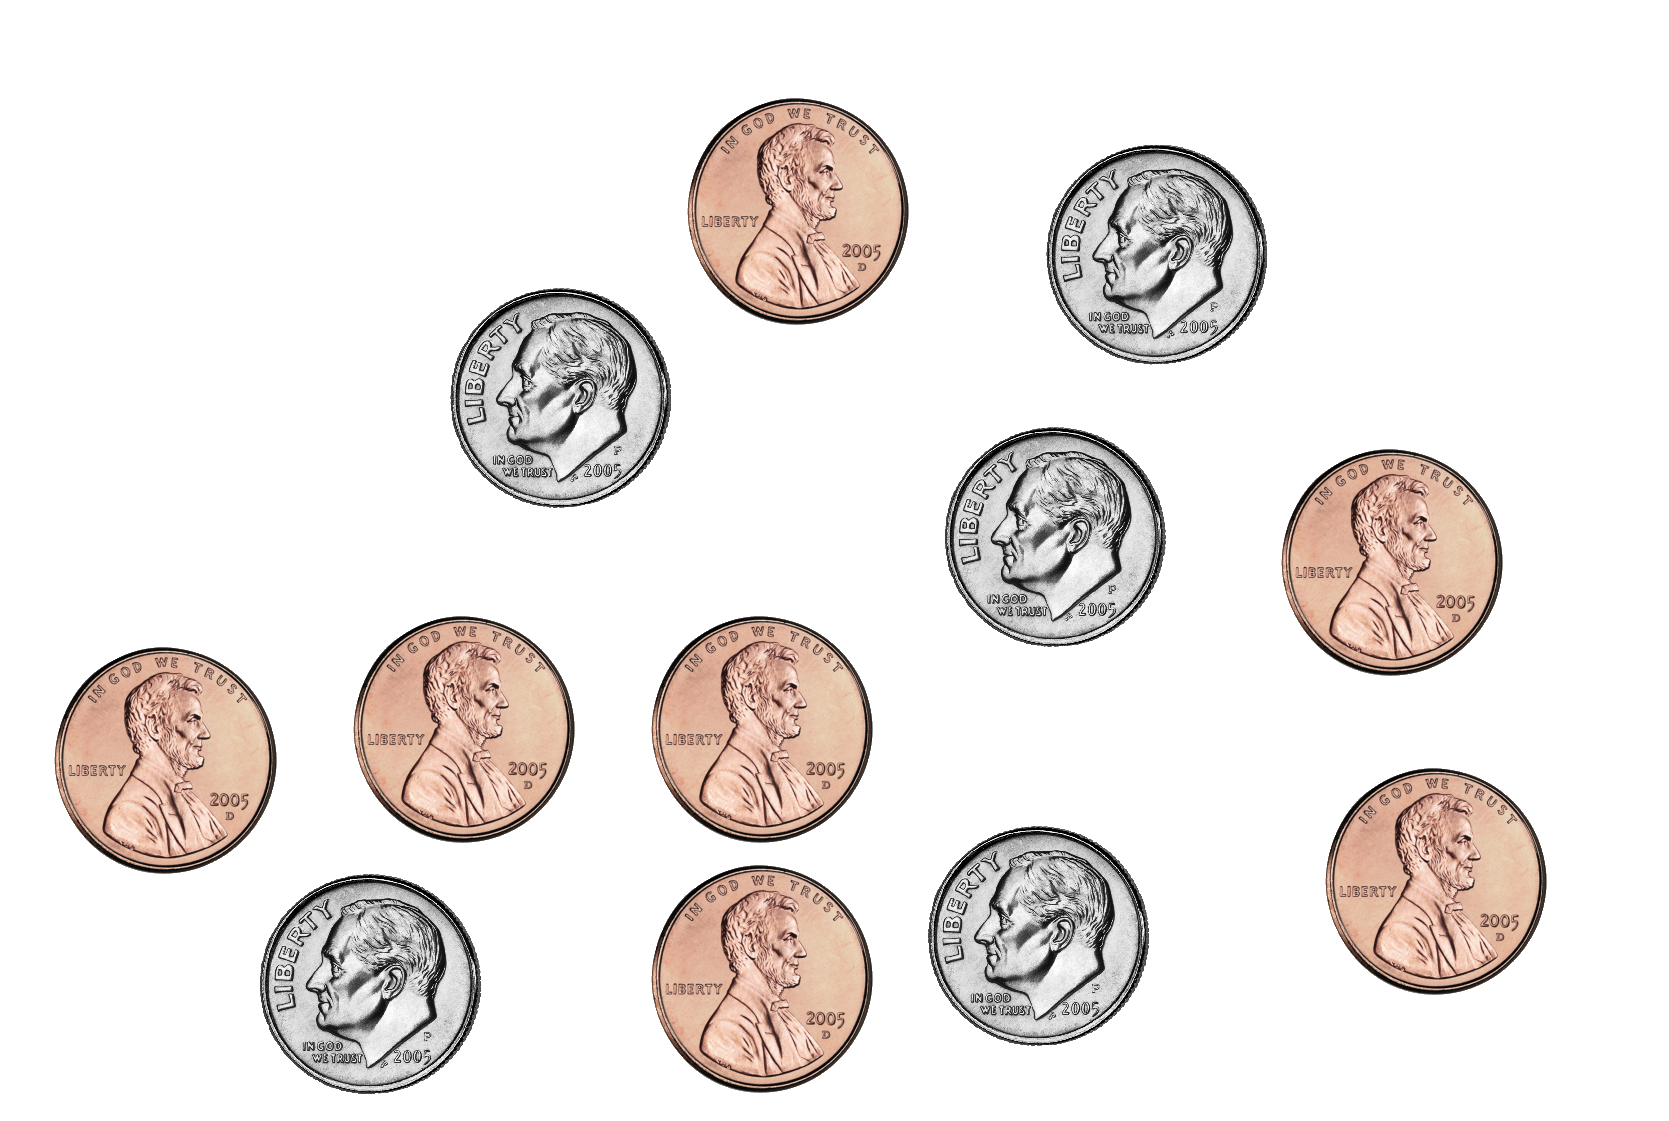
\includegraphics[height=1in]{takeawayCoins/12.pdf}
  }
\end{frame}

\begin{frame}
  \textbf{Proof:} Player $\pl B$ can always end her round so that there's $8$,
  then $4$, then $0$ coins. For example:

  \vpause

  {\small \begin{center}\begin{tabular}{cc}
    $12-1=11$ & $11-3=8$ \\
    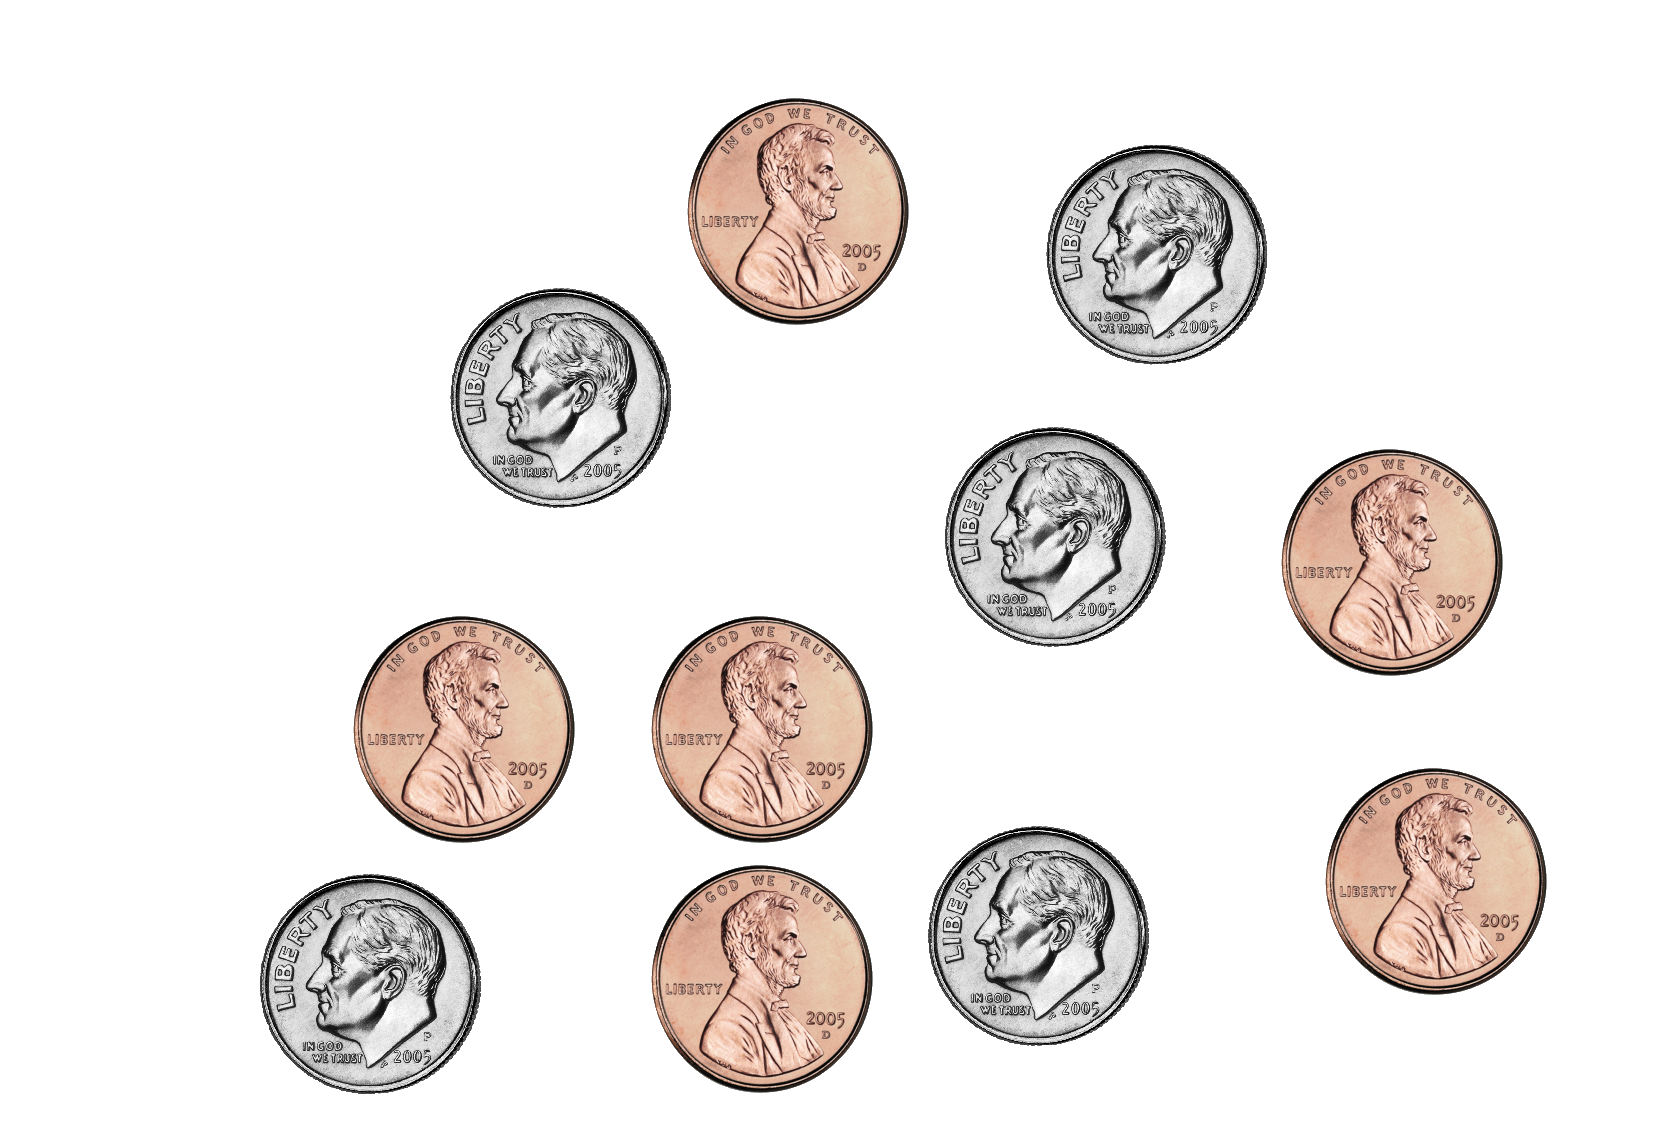
\includegraphics[height=0.5in]{takeawayCoins/11.pdf} &
    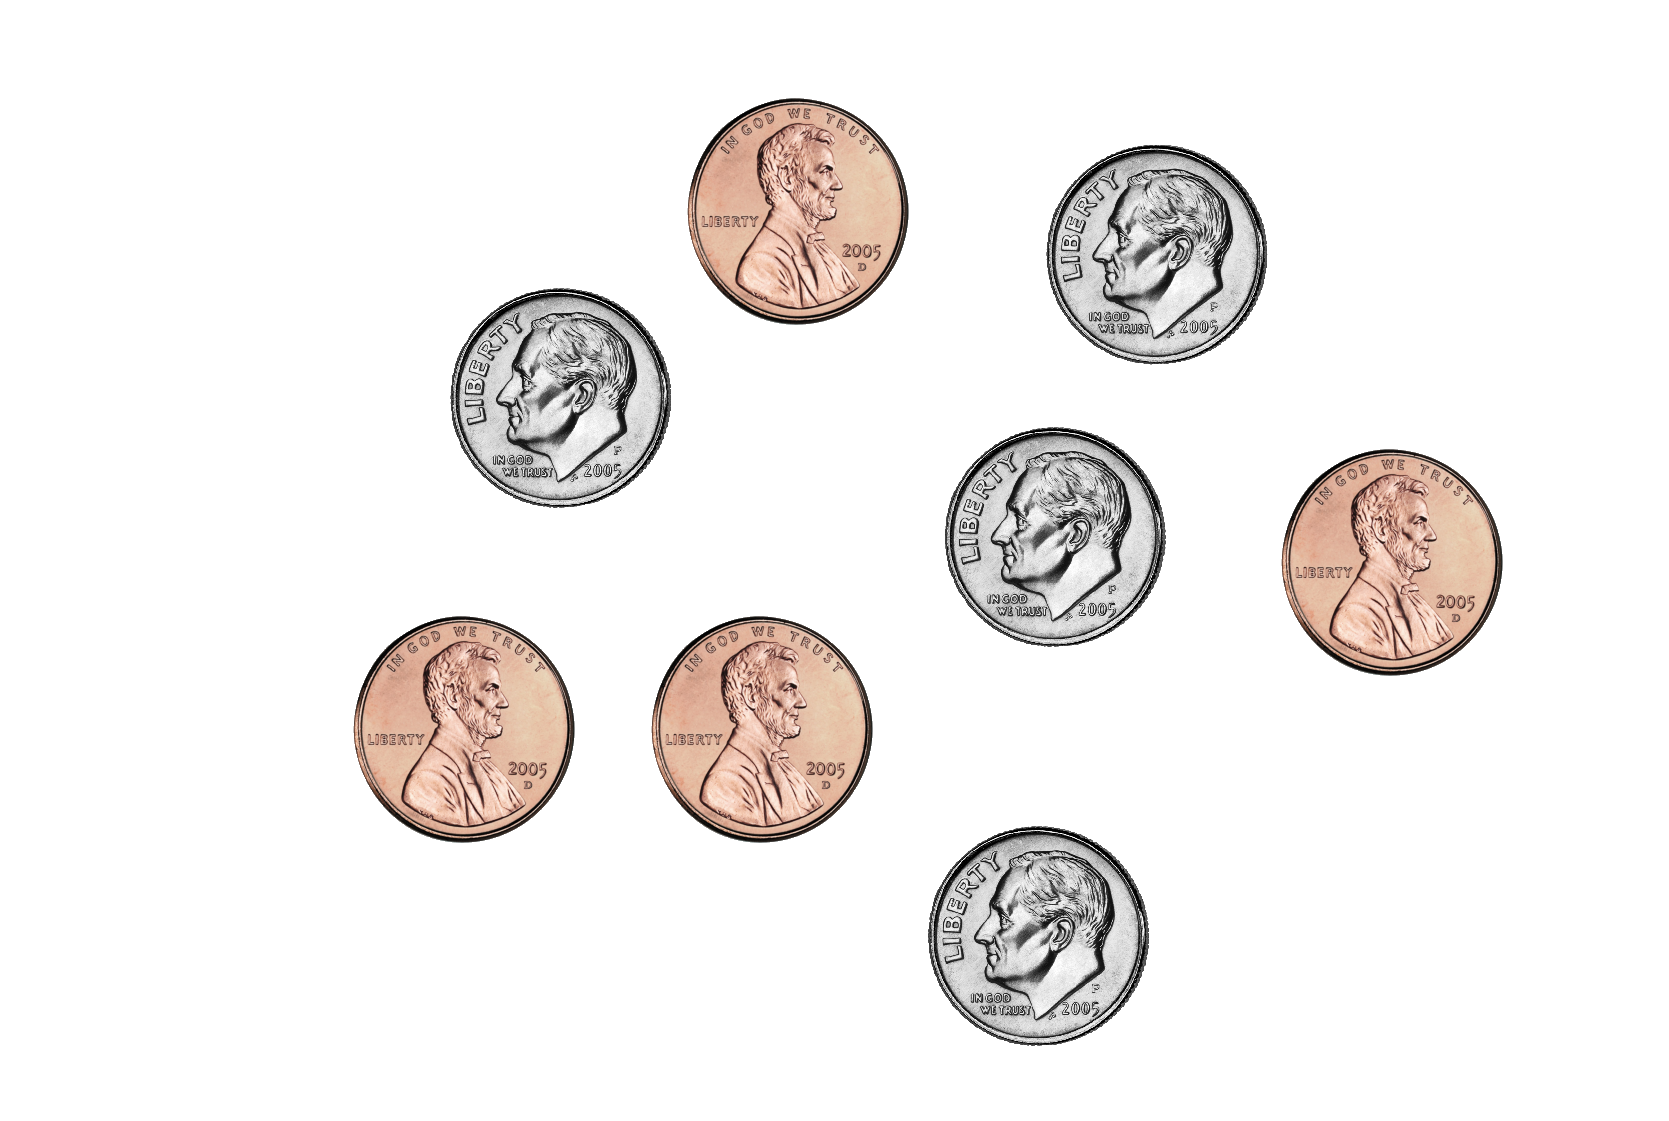
\includegraphics[height=0.5in]{takeawayCoins/08.pdf} \vspace{1em}\\

    $12-2=10$ & $10-2=8$ \\
    
\includegraphics[height=0.5in]{takeawayCoins/10.pdf} &
    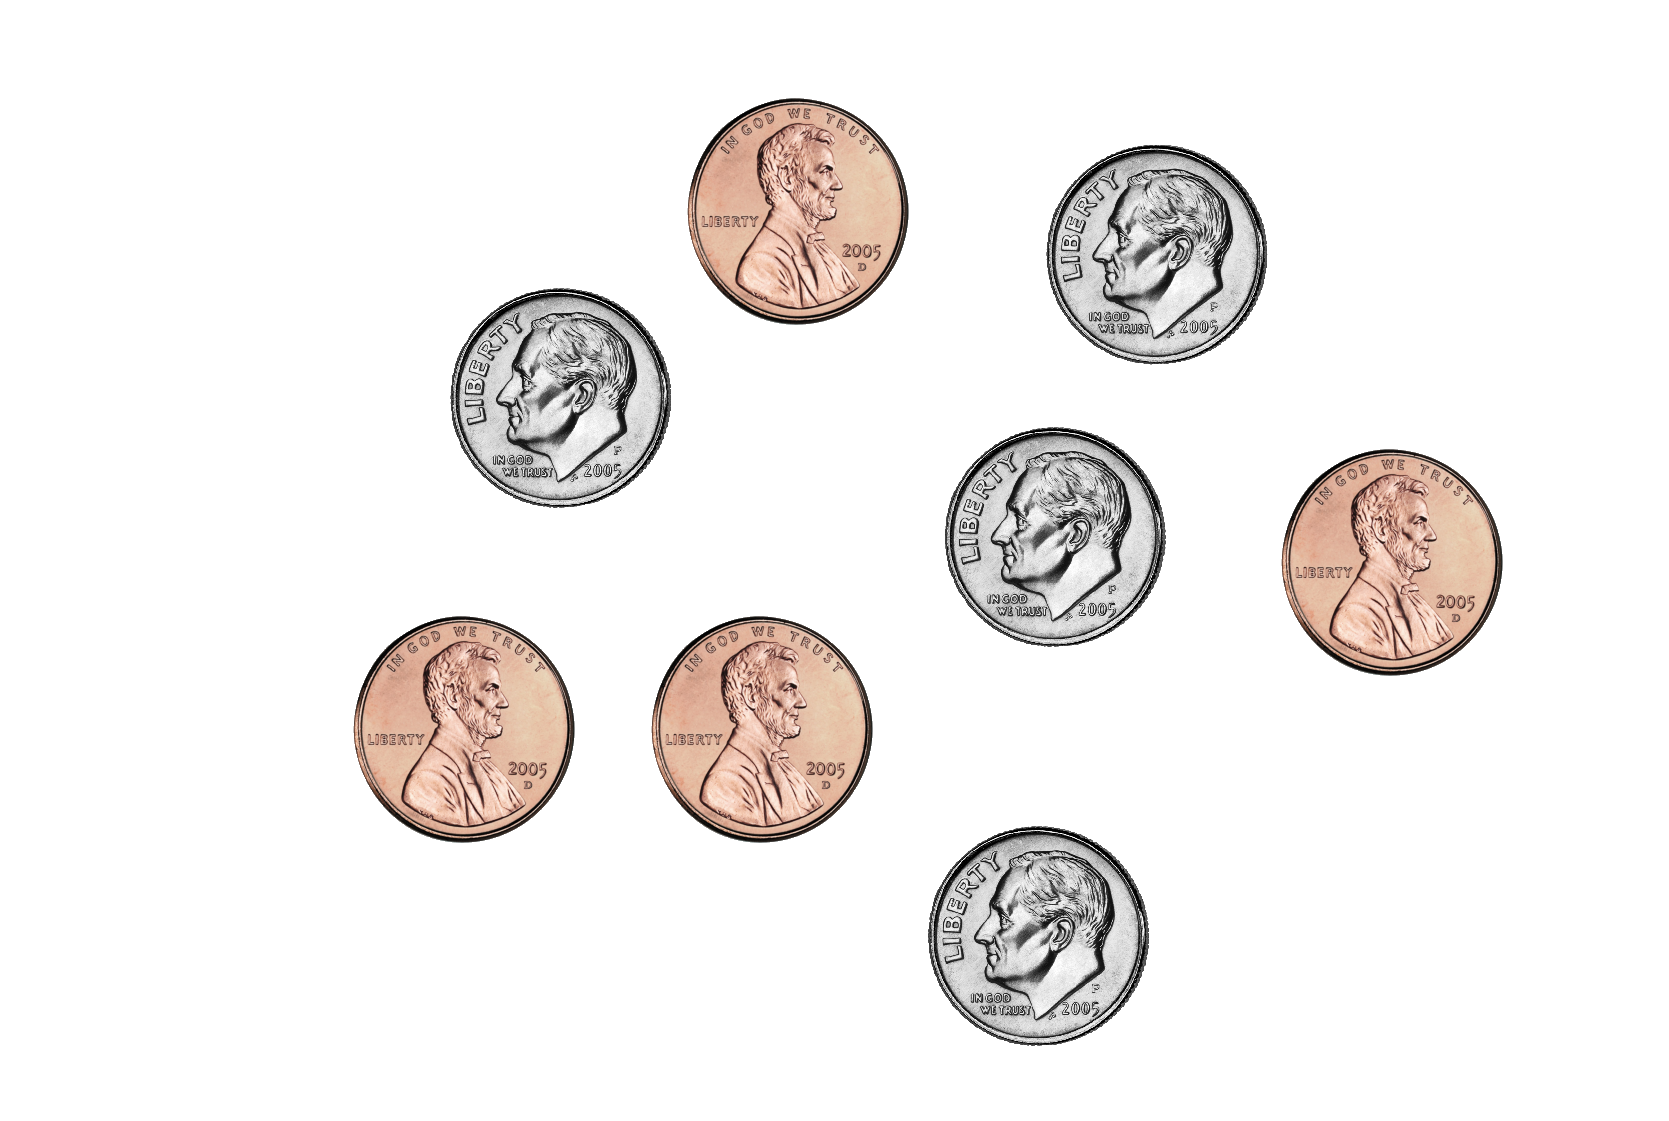
\includegraphics[height=0.5in]{takeawayCoins/08.pdf} \vspace{1em}\\

    $12-3=9$ & $9-1=8$ \\
    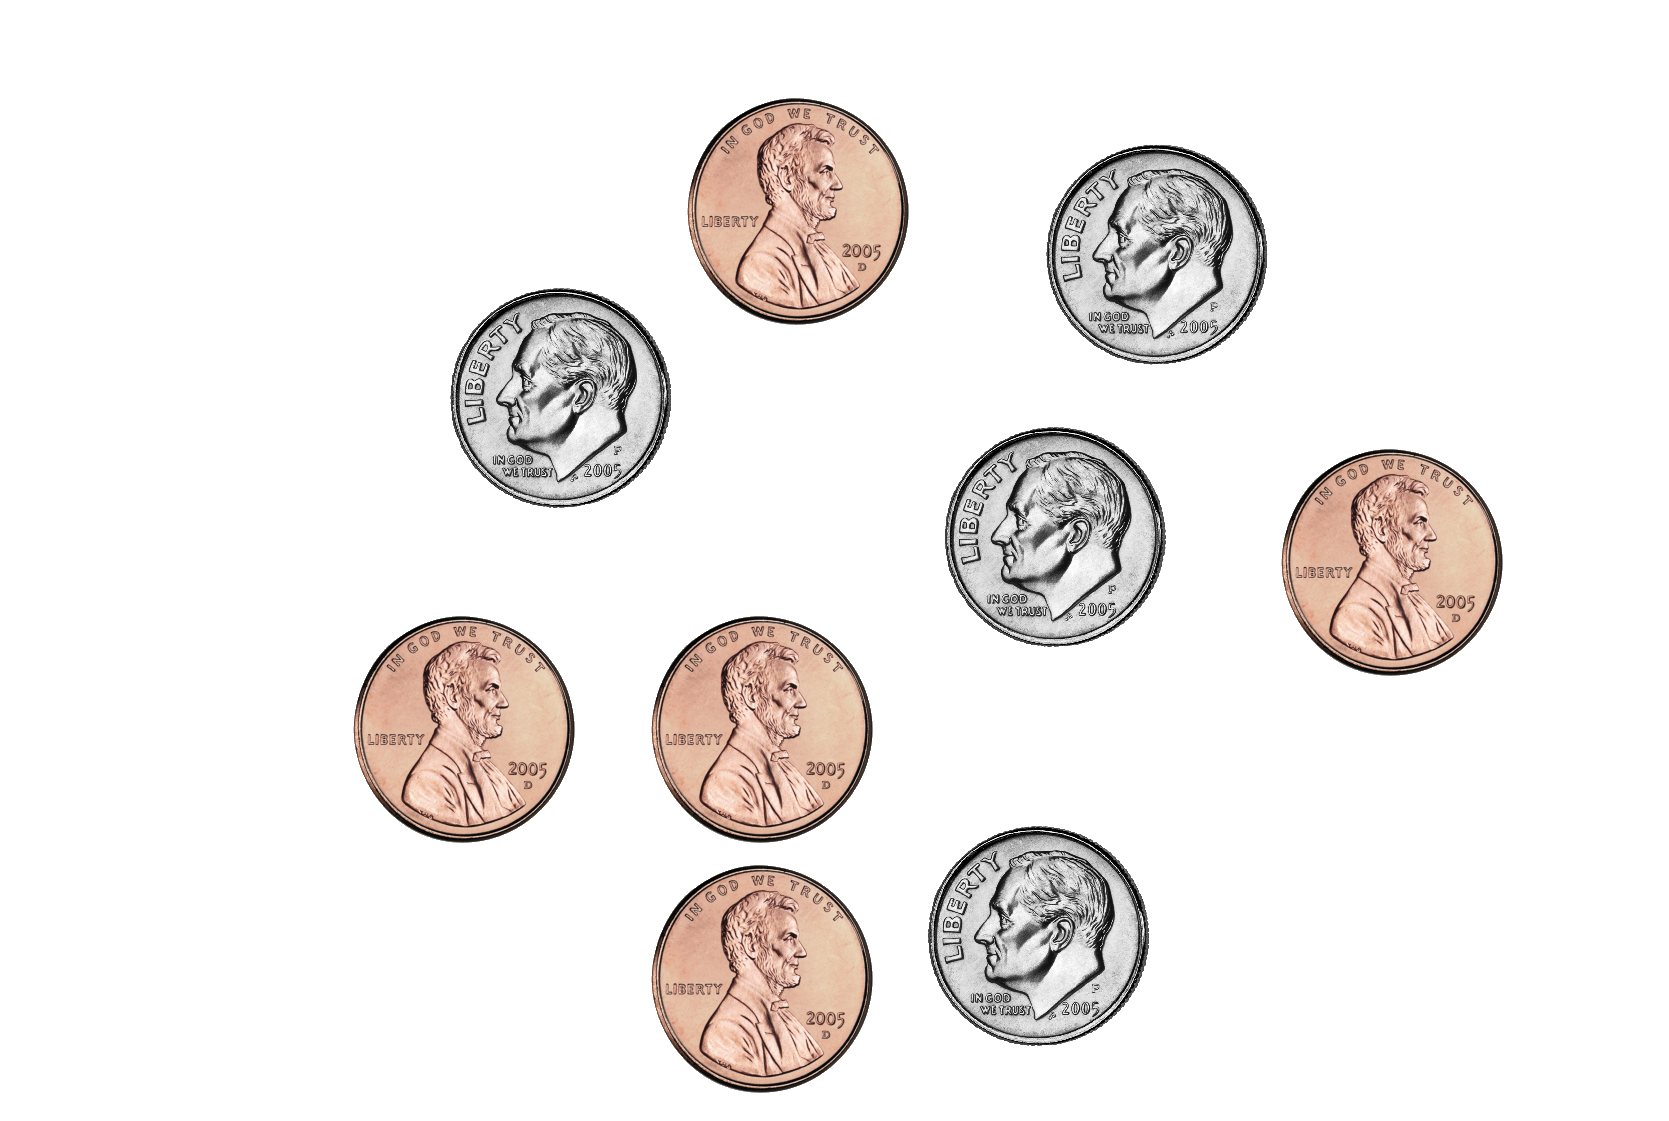
\includegraphics[height=0.5in]{takeawayCoins/09.pdf} &
    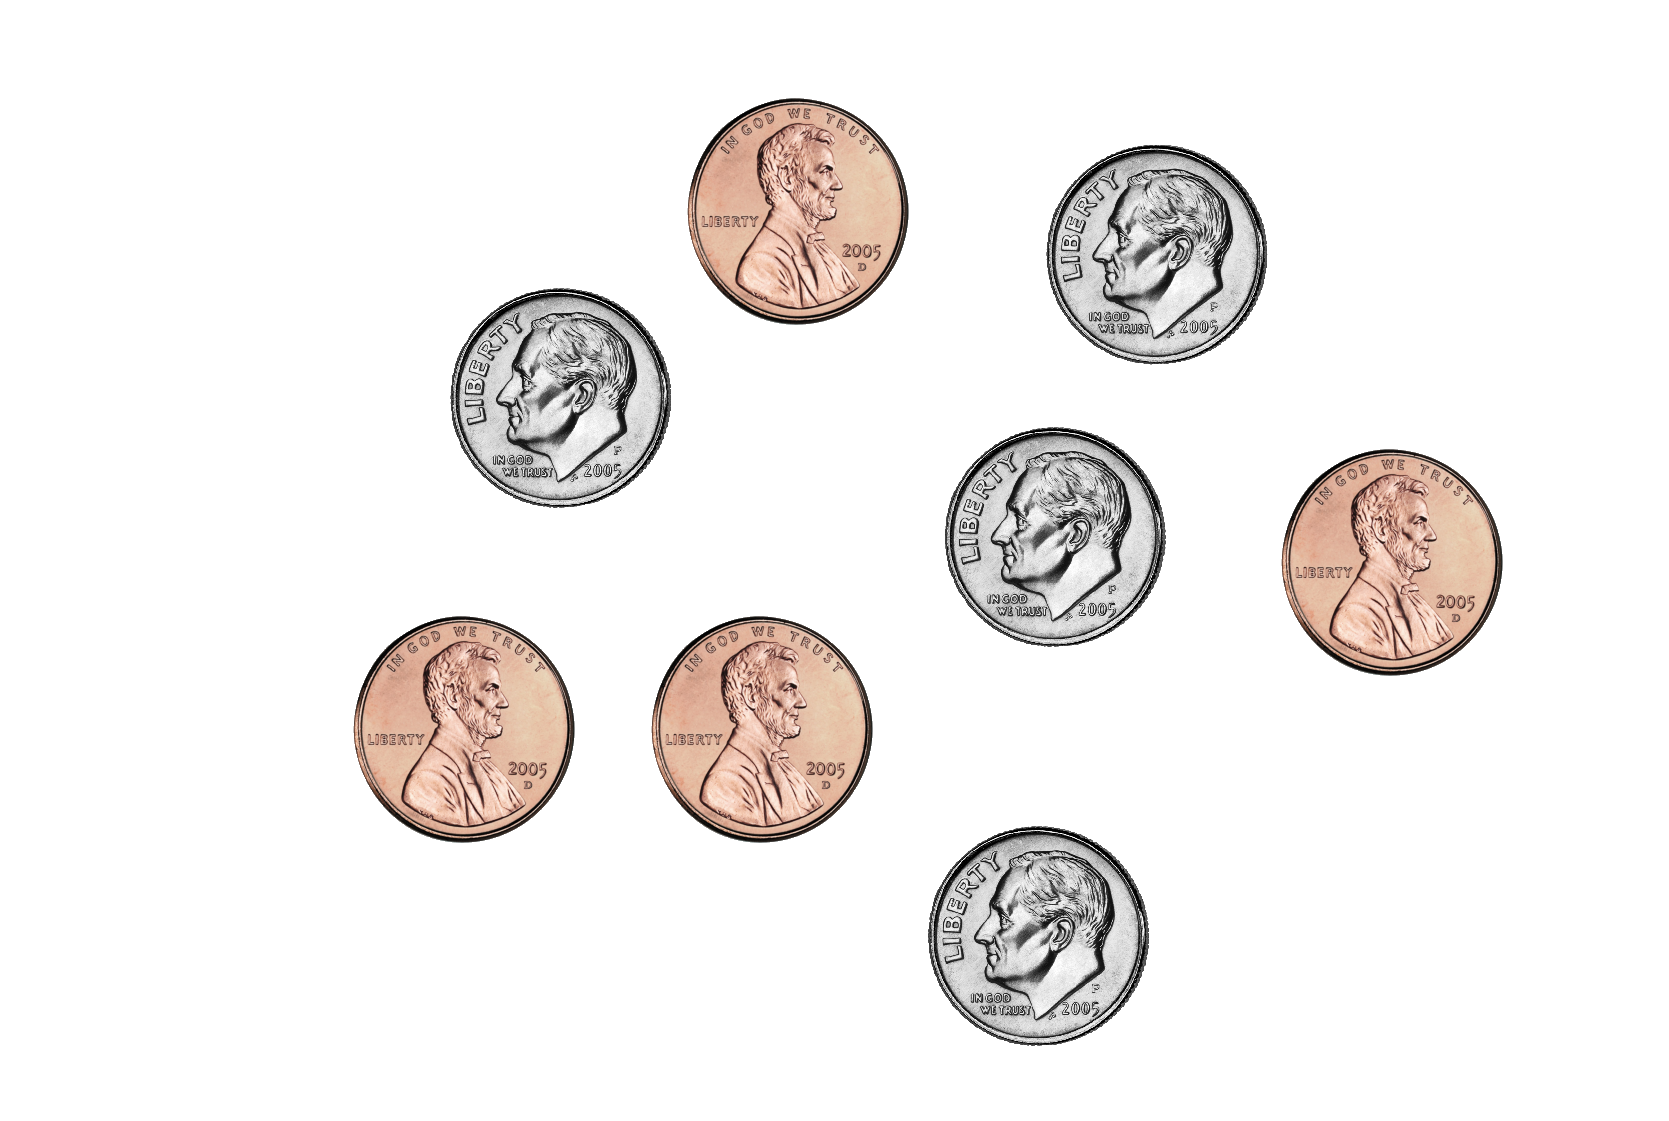
\includegraphics[height=0.5in]{takeawayCoins/08.pdf} \\
  \end{tabular}\end{center} }

\end{frame}

\begin{frame}
  Two puzzles to try out.

  \vpause

  \textbf{Puzzle 1:} Show that Player $\pl A$ had a winning strategy
  in Takeaway played with $15$ coins (which she obviously didn't follow
  in the example).

  \vpause

  \textbf{Puzzle 2:} Make a general rule about the number of starting coins
  which tells whether Player $\pl A$ or $\pl B$ has a winning strategy in
  Takeaway.
\end{frame}

\subsection{Nim}

\begin{frame}{Nim}
  In \term{Nim}, the Players $\pl A$, $\pl B$ take turns removing $1$ or more
  coins from the table, but cannot take more than one type of coin at a
  time. The player who removes the last coin wins.

  \vspace{1em}

  \centerline{
    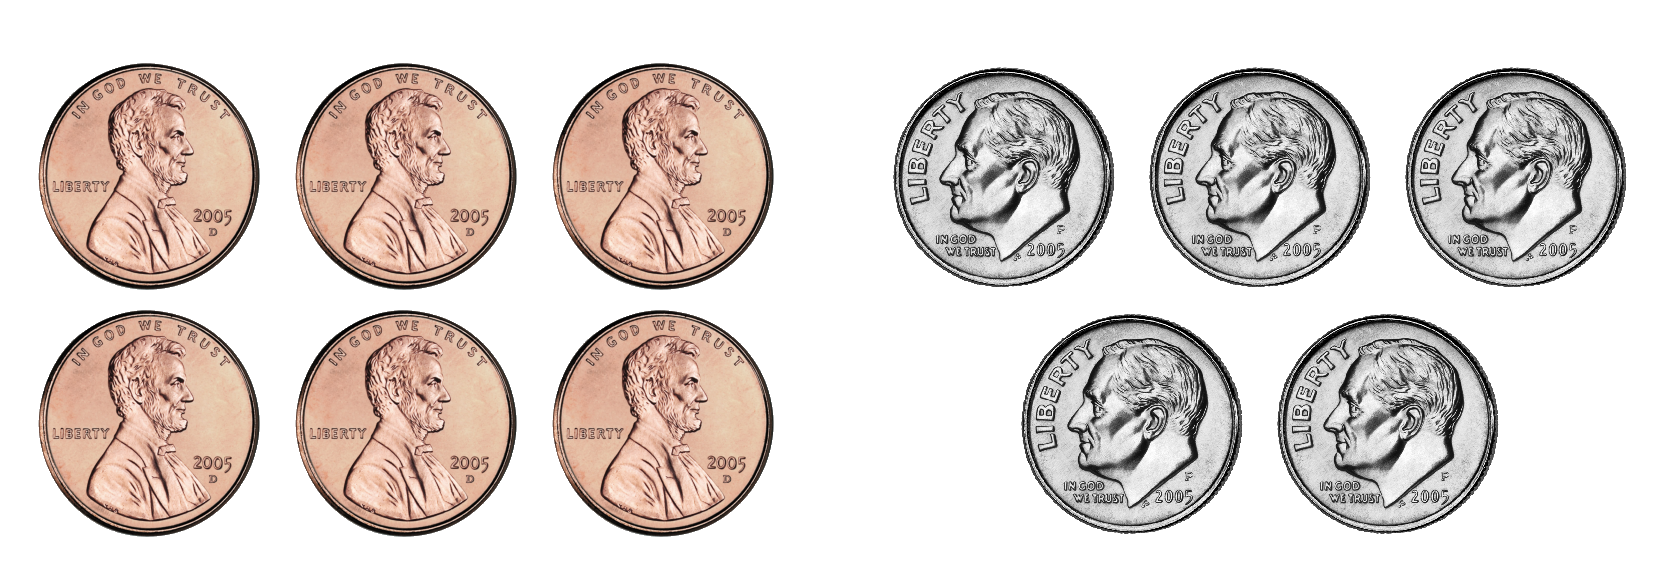
\includegraphics[height=1.7in]{nimCoins/65.pdf}
  }
\end{frame}

\begin{frame}
  Round 1a: Player $\pl A$ takes away 3 pennies.

  \centerline{
    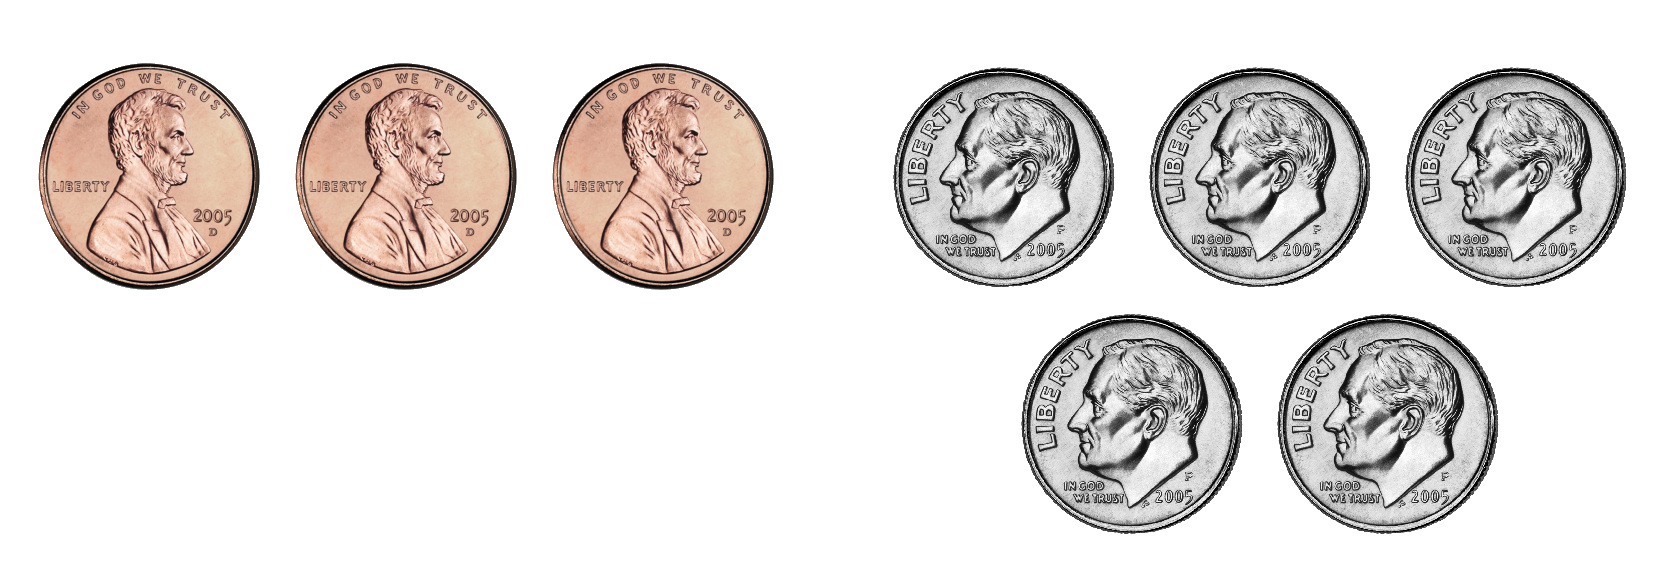
\includegraphics[height=1.7in]{nimCoins/35.pdf}
  }
\end{frame}


\begin{frame}
  Round 1b: Player $\pl B$ takes away 1 dime.

  \centerline{
    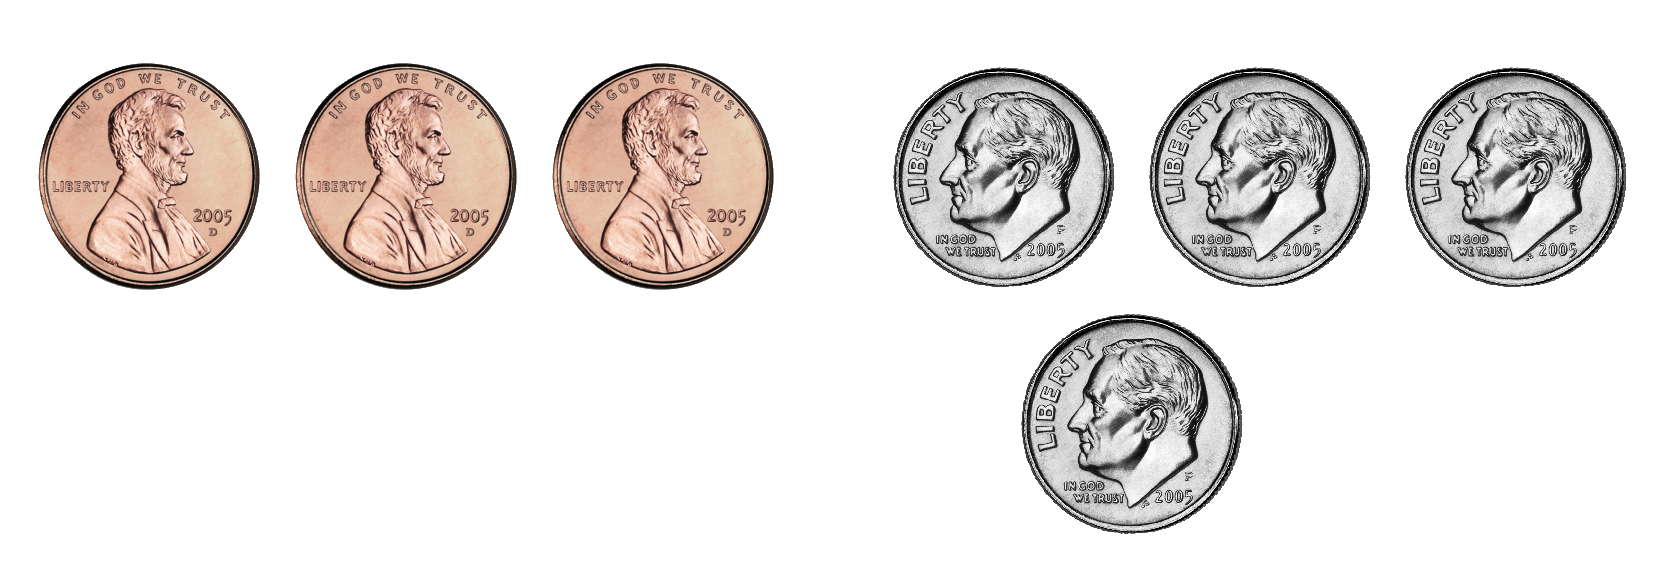
\includegraphics[height=1.7in]{nimCoins/34.pdf}
  }
\end{frame}


\begin{frame}
  Round 2a: Player $\pl A$ takes away 2 dimes.

  \centerline{
    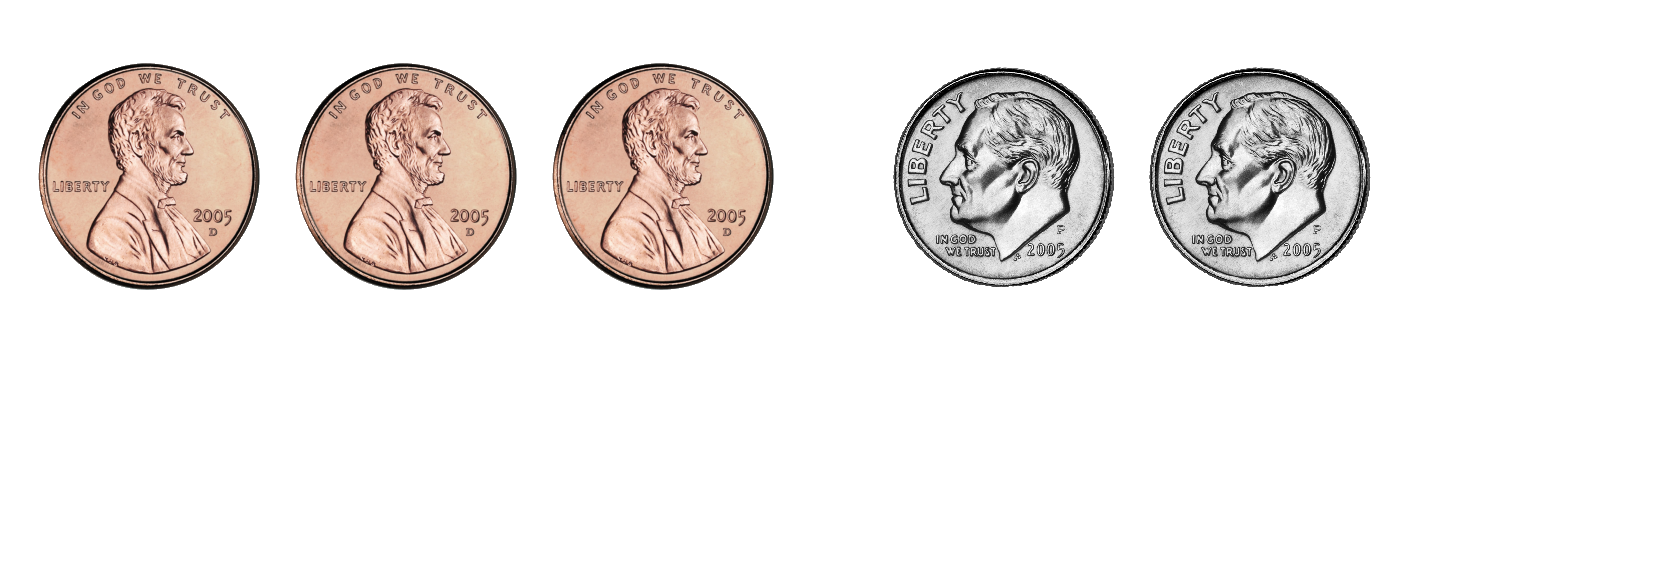
\includegraphics[height=1.7in]{nimCoins/32.pdf}
  }
\end{frame}


\begin{frame}
  Round 2b: Player $\pl B$ takes away 2 pennies.

  \centerline{
    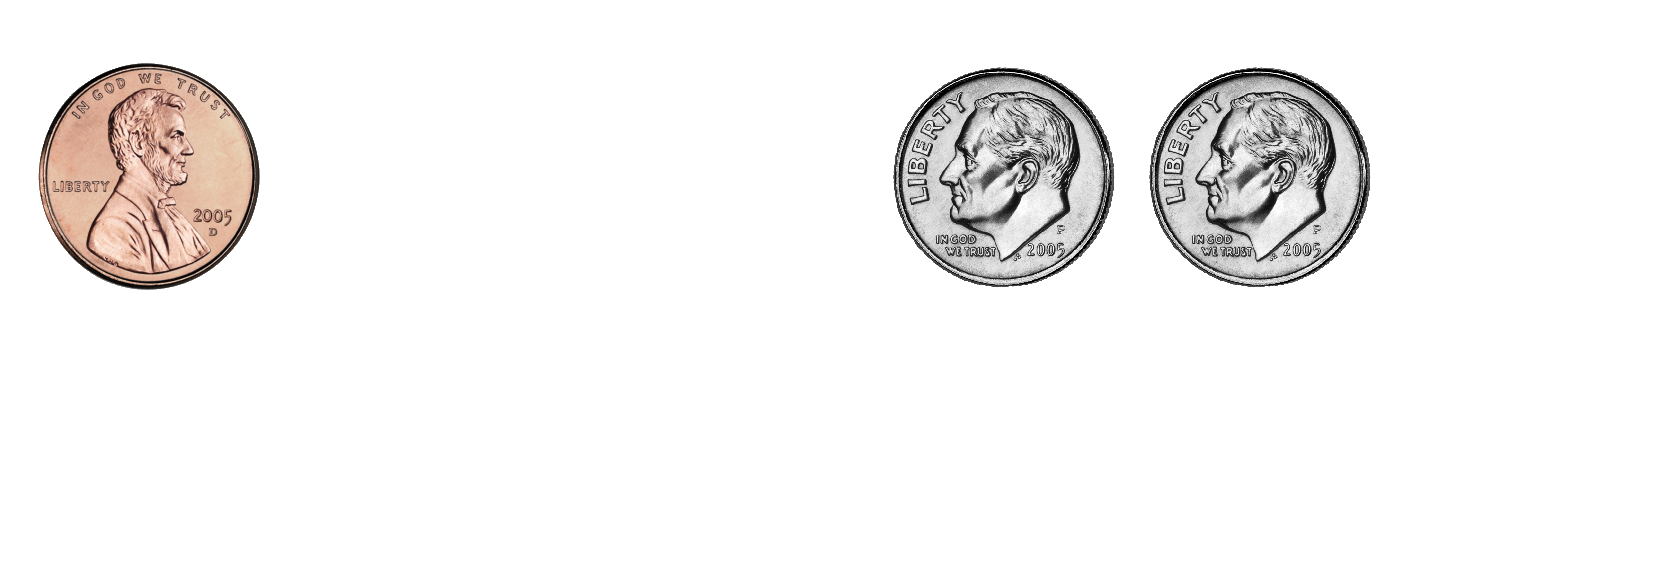
\includegraphics[height=1.7in]{nimCoins/12.pdf}
  }
\end{frame}


\begin{frame}
  Round 3a: Player $\pl A$ takes away the last penny.

  \centerline{
    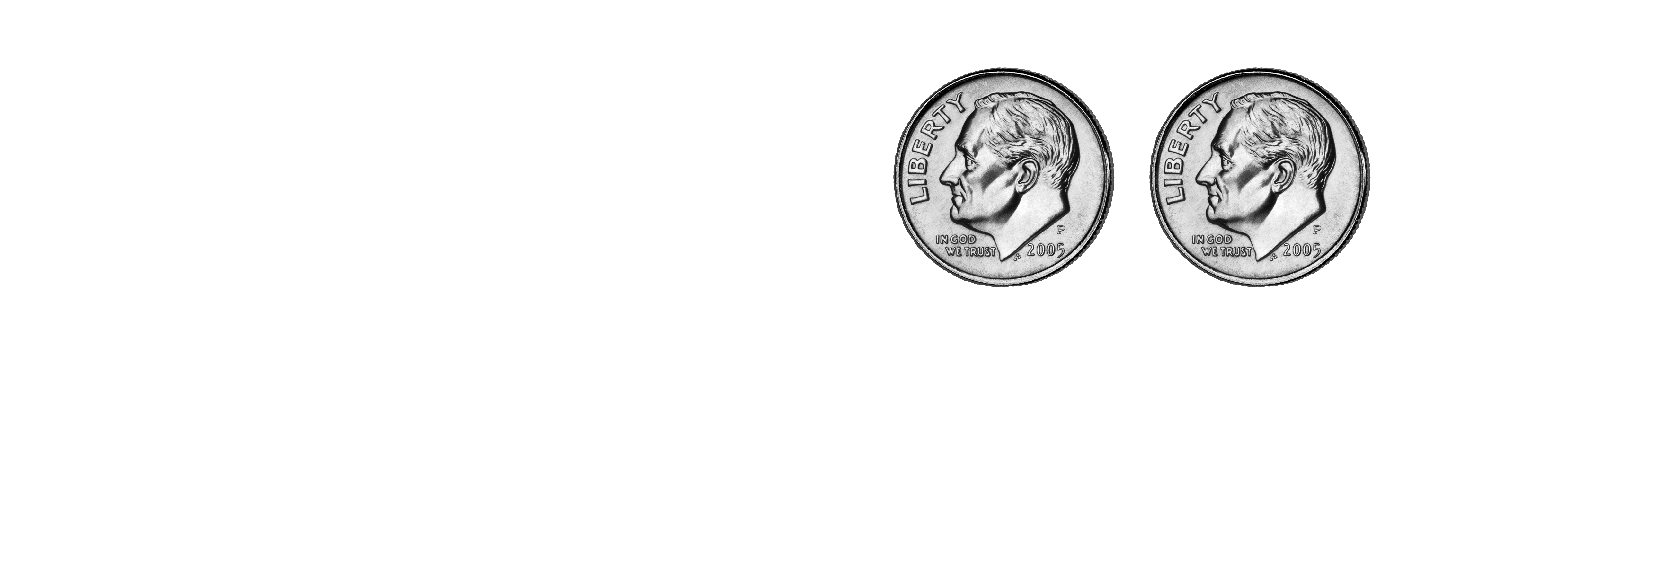
\includegraphics[height=1.7in]{nimCoins/02.pdf}
  }
\end{frame}


\begin{frame}
  Round 3b: Player $\pl B$ takes away the last 2 dimes, and wins!

  \centerline{
    
\includegraphics[height=1.7in]{nimCoins/00.pdf}
  }
\end{frame}

\begin{frame}{A winning strategy}
  Just like in Takeaway, we want to know when each player has a winning
  strategy which guarantees that they cannot lose the game.

  \vpause

  I claim that when Takeaway starts with $4$ pennies and $4$ dimes, then Player
  $\pl B$ has a winning strategy.

  \centerline{
    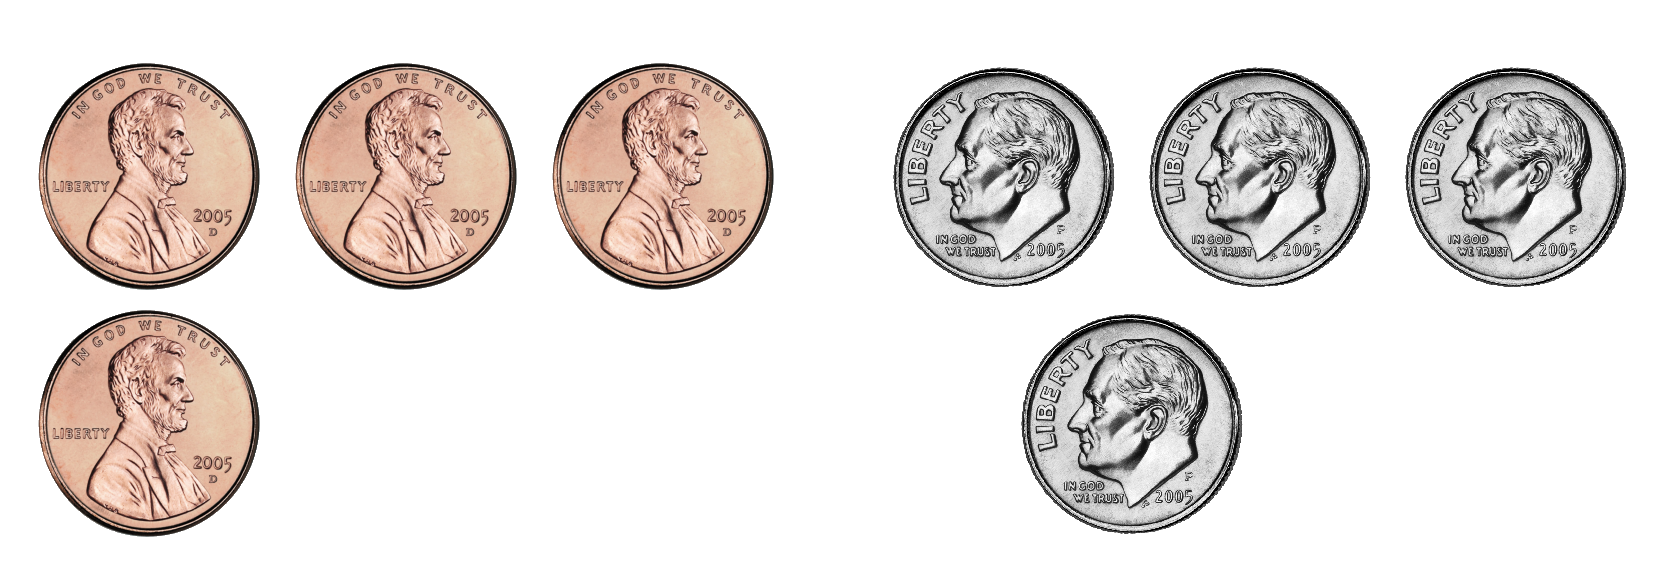
\includegraphics[height=1in]{nimCoins/44.pdf}
  }
\end{frame}

\begin{frame}
  \textbf{Proof:} Player $\pl B$ can always end her round so that there's the
  same number of coins in both piles.

  \vpause

  {\small \begin{center}\begin{tabular}{cc}
    $(2,4)$ & $(2,2)$ \\
    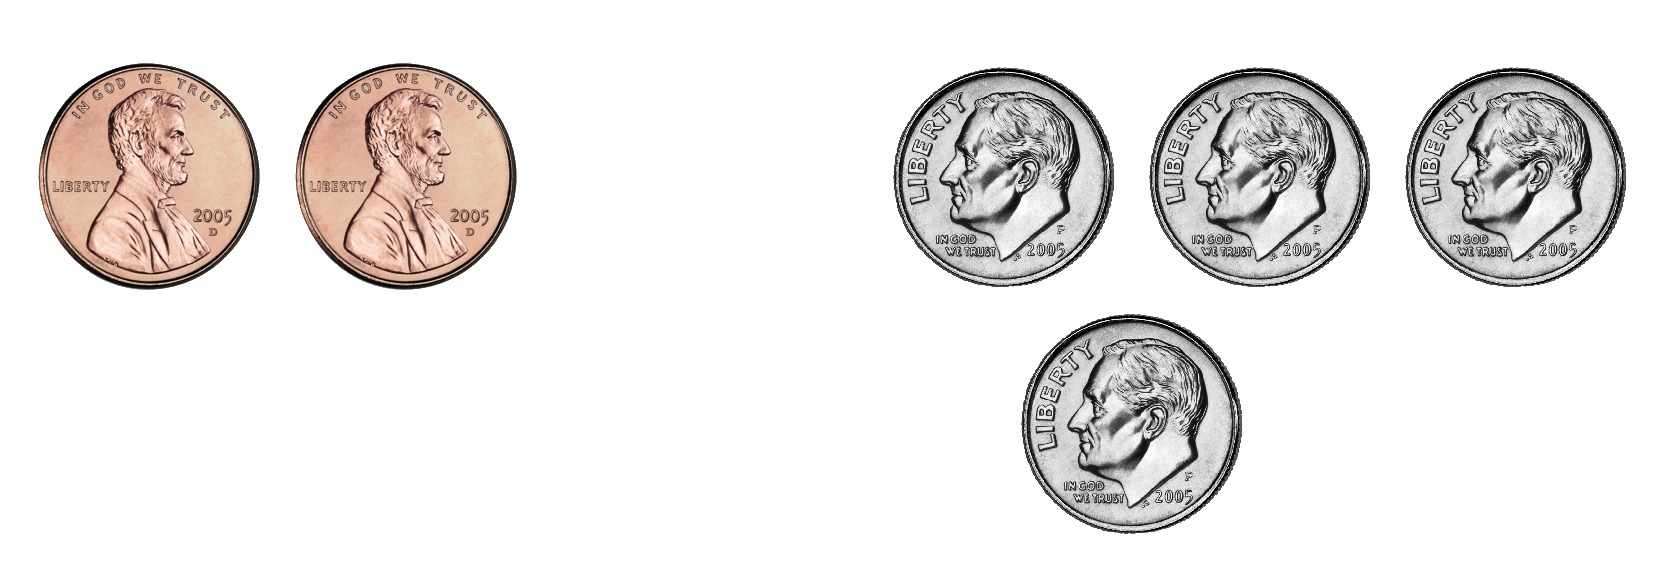
\includegraphics[height=0.5in]{nimCoins/24.pdf} &
    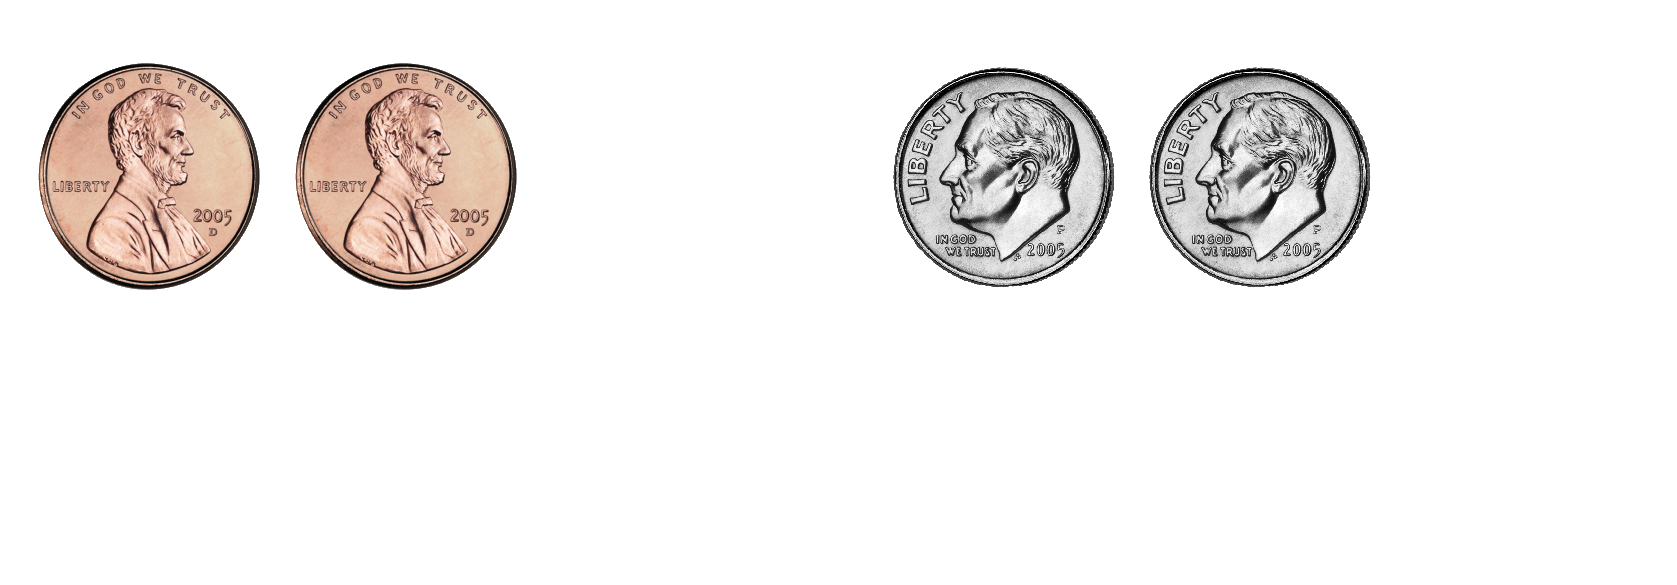
\includegraphics[height=0.5in]{nimCoins/22.pdf} \vspace{1em}\\

    $(4,1)$ & $(1,1)$ \\
    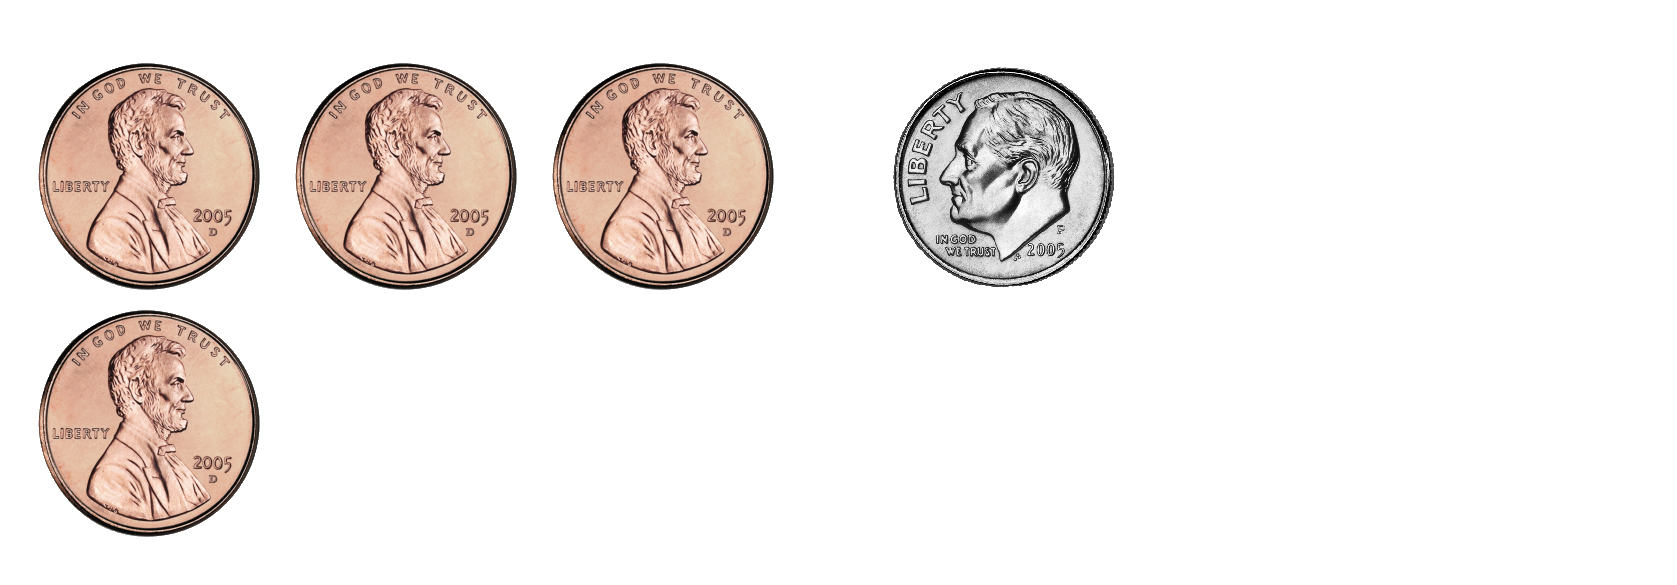
\includegraphics[height=0.5in]{nimCoins/41.pdf} &
    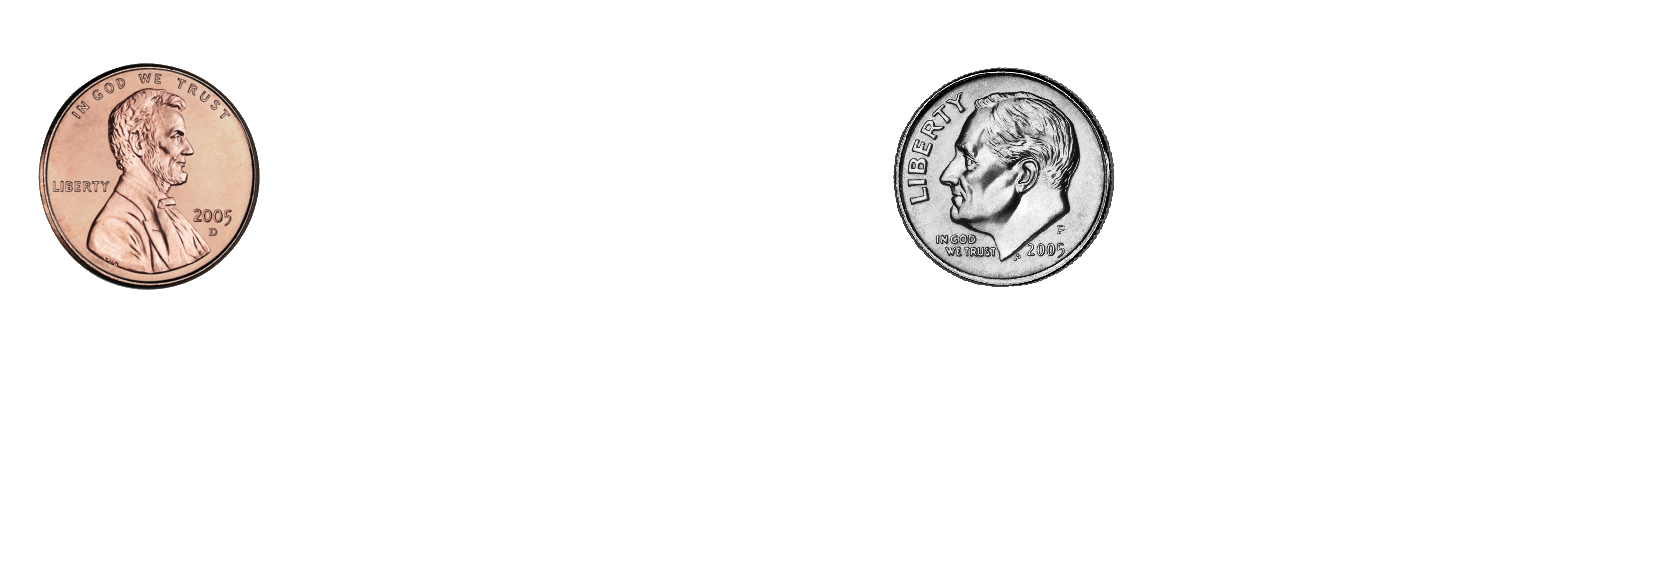
\includegraphics[height=0.5in]{nimCoins/11.pdf} \vspace{1em}\\

    $(3,4)$ & $(3,3)$ \\
    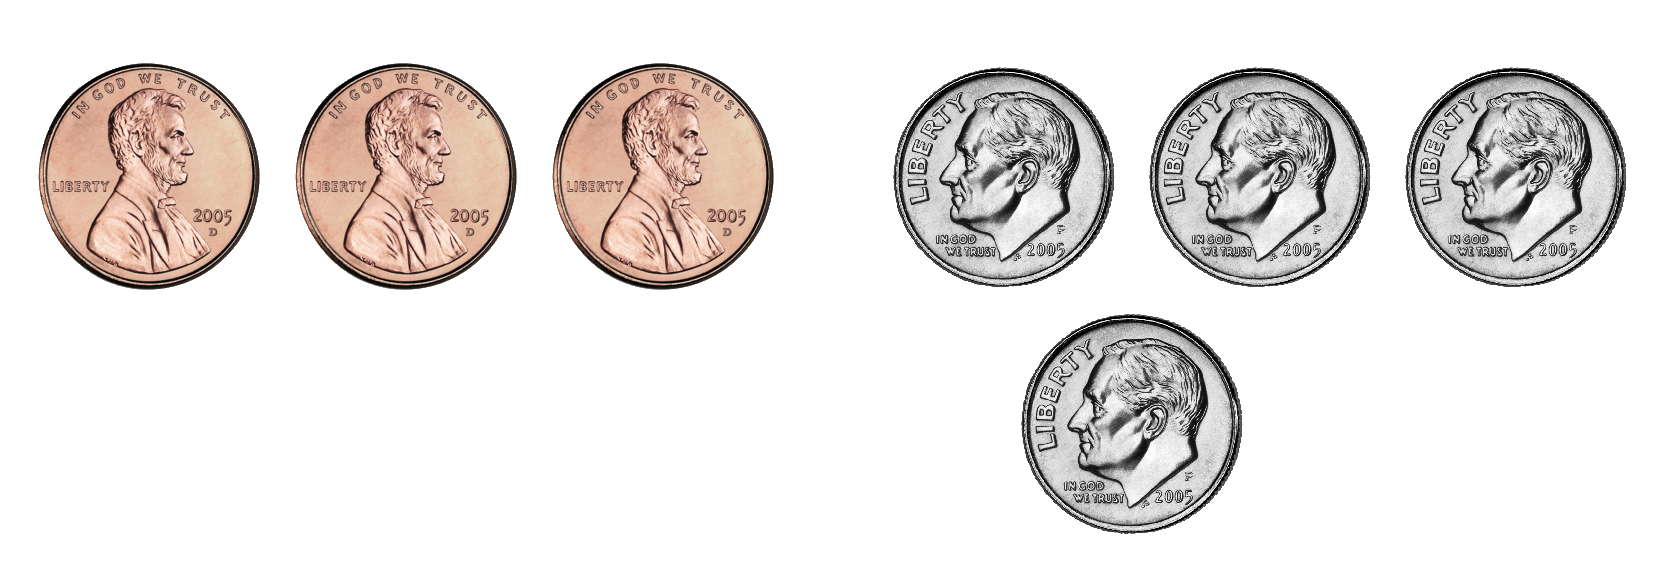
\includegraphics[height=0.5in]{nimCoins/34.pdf} &
    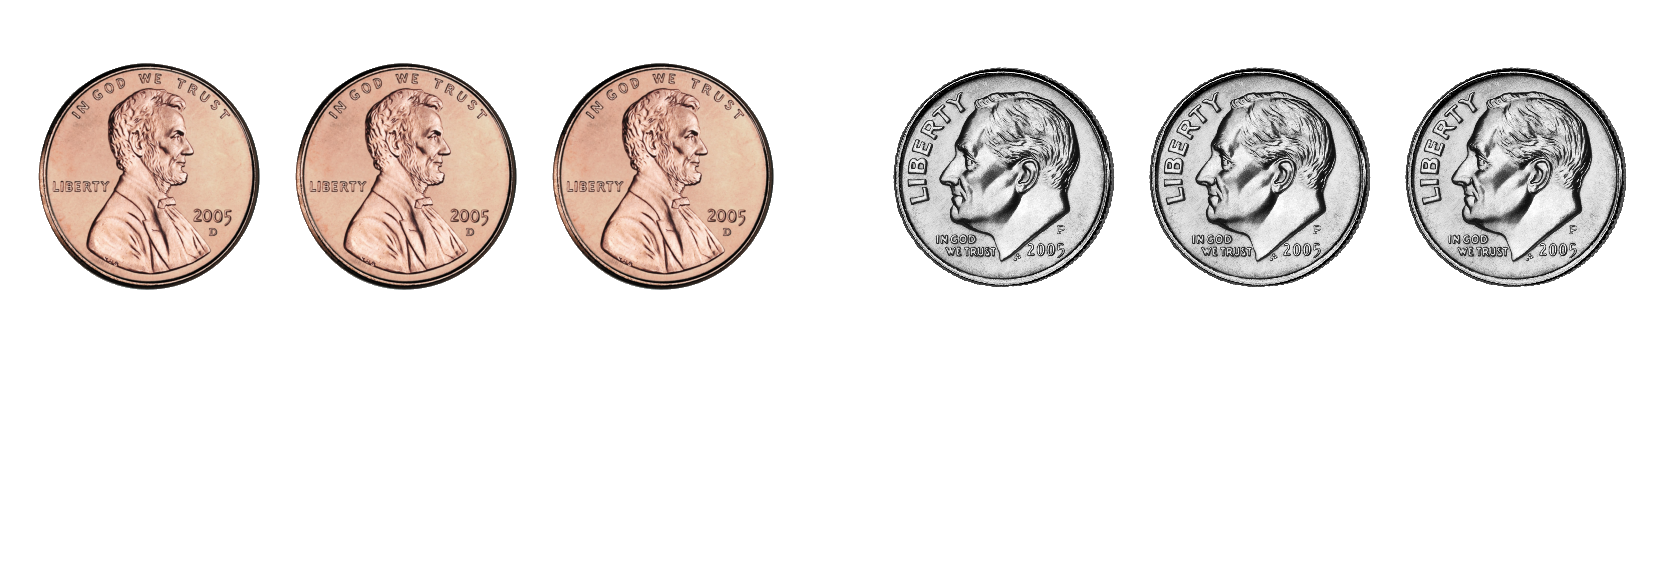
\includegraphics[height=0.5in]{nimCoins/33.pdf} \\
  \end{tabular}\end{center} }

\end{frame}

\begin{frame}
  Three more puzzles!

  \vpause

  \textbf{Puzzle 3:} Show that Player $\pl A$ had a winning strategy
  in Takeaway played with $6$ pennies and $5$ dimes (which she obviously
  didn't follow in the example).

  \vpause

  \textbf{Puzzle 4:} Make a general rule about the number of starting pennies
  and dimes which tells whether Player $\pl A$ or $\pl B$ has a winning
  strategy in Nim.

  \vpause

  \textbf{Puzzle 5:} Investigate how the game changes if more types of coins
  are allowed.
\end{frame}

\section{Finding Winning Strategies}

\subsection{Modeling Arbitrary Games}

\begin{frame}{Decision Trees}
  Since our games involve two players making decisions, we can model them
  by drawing a tree which maps all possible sequences of decisions (known
  as \term{extensive form}).

  \centerline{
    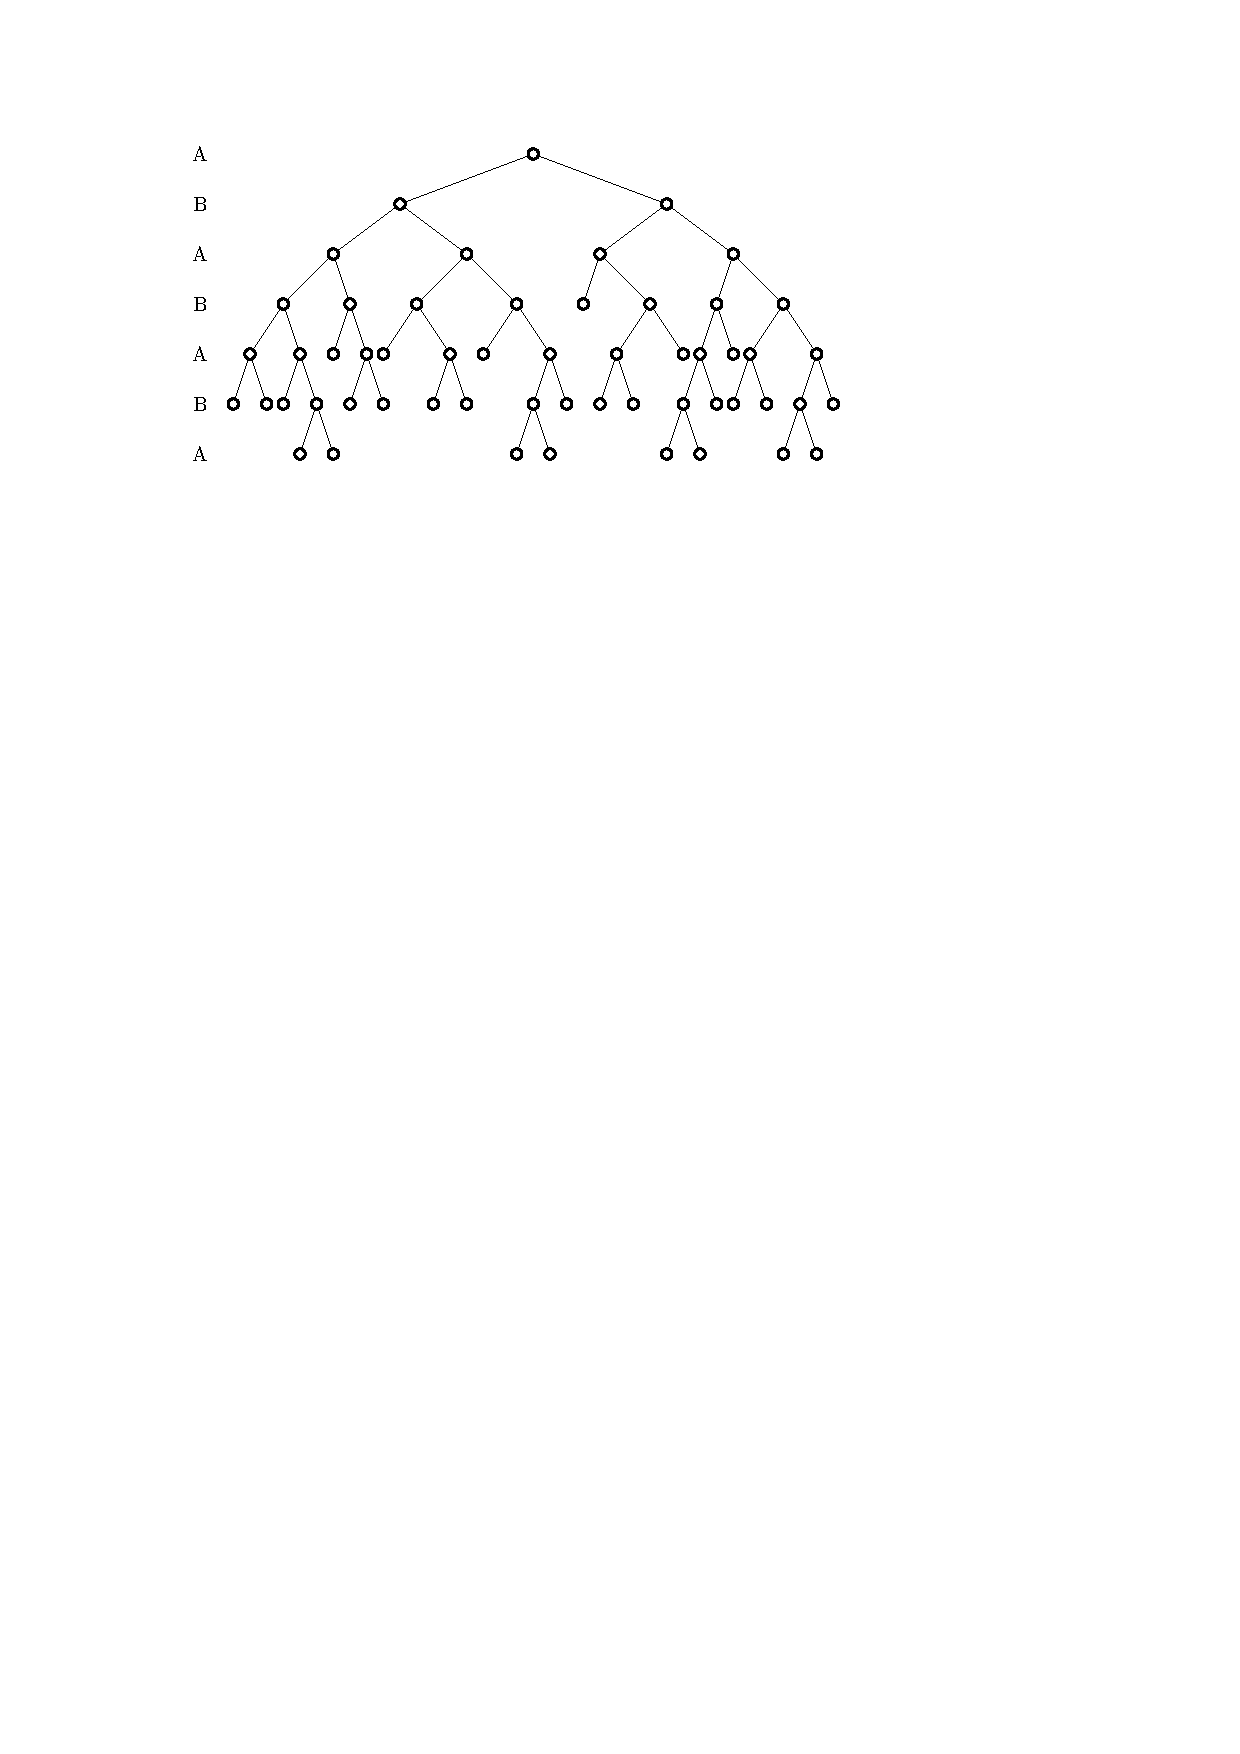
\includegraphics[height=1.5in]{decisionTree1.pdf}
  }

  The player which starts their turn in a bottom node loses the game.
  (We assume no ties.)
\end{frame}

\subsection{Zermelo's Theorem}

\begin{frame}{Zermelo's Theorem}
  \term{Zermelo's Theorem} states that for every two-player sequential game
  of finite length, one of the players has a winning strategy which can be
  discovered by ``backwards induction'' on its decision tree.
\end{frame}


\begin{frame}
  \centerline{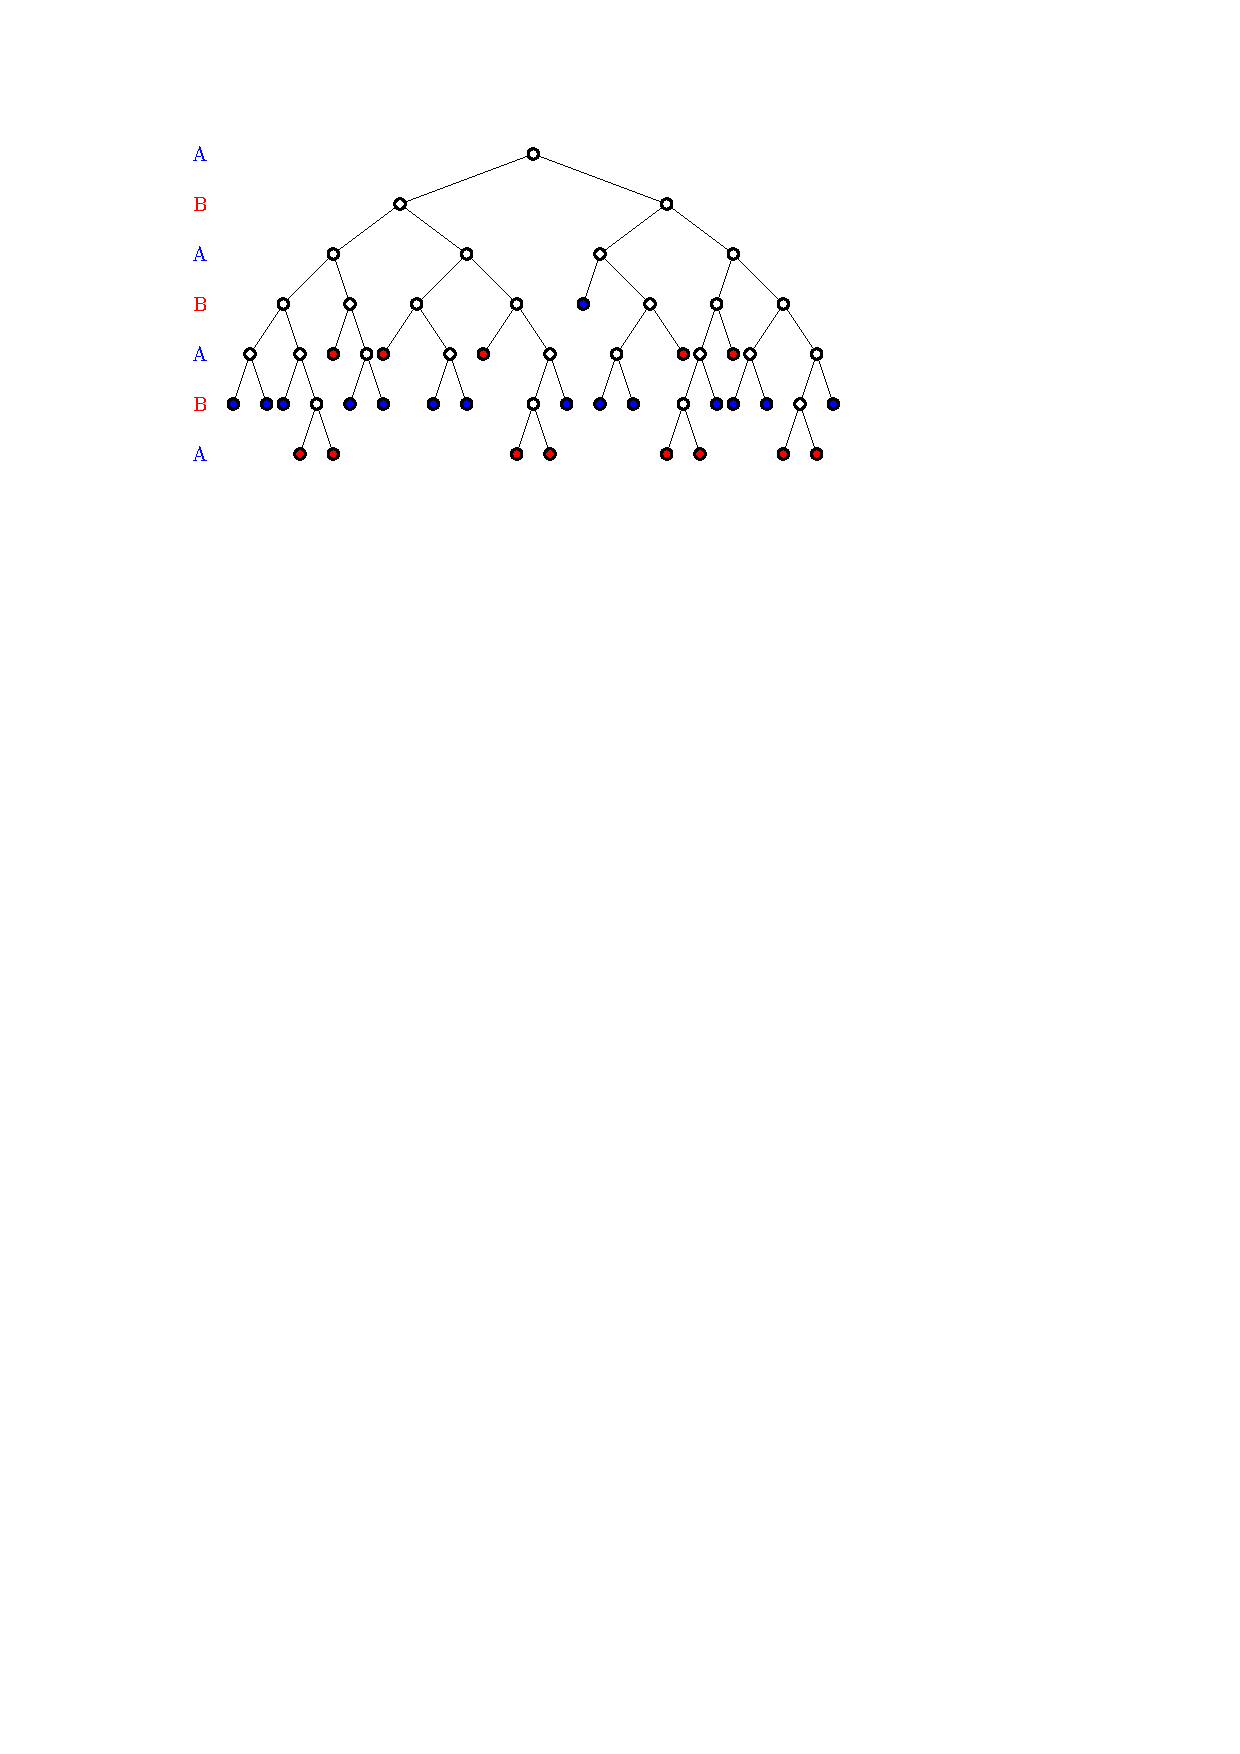
\includegraphics[width=3in]{decisionTree2.pdf}}

  \vspace{1em}

  Label the tree by first showing the states where $\pl A$ (blue) and
  $\pl B$ (red) have already won the game.
\end{frame}

\begin{frame}
  \centerline{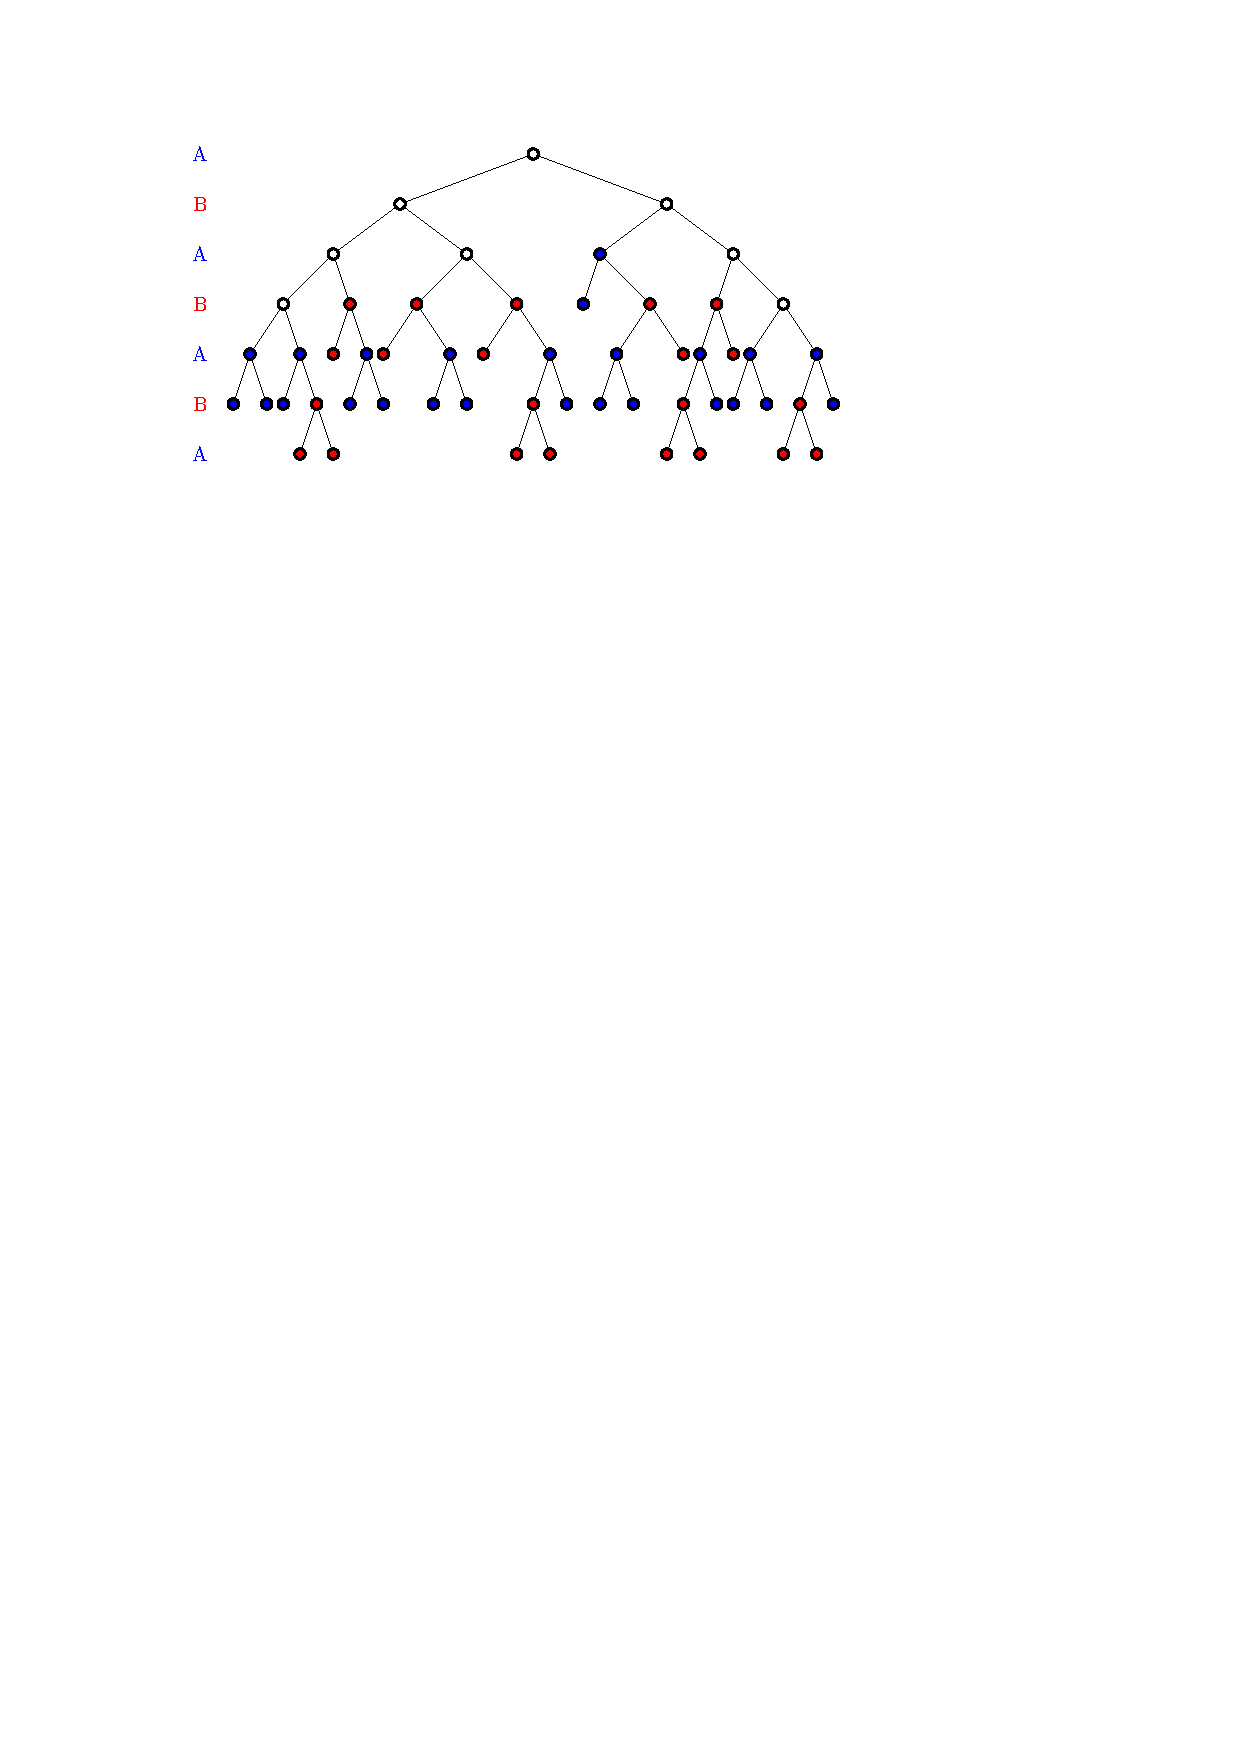
\includegraphics[width=3in]{decisionTree3.pdf}}

  \vspace{1em}

  Then move back and label the spaces where the active player is able
  to move to a vertex of their color.
\end{frame}

\begin{frame}
  \centerline{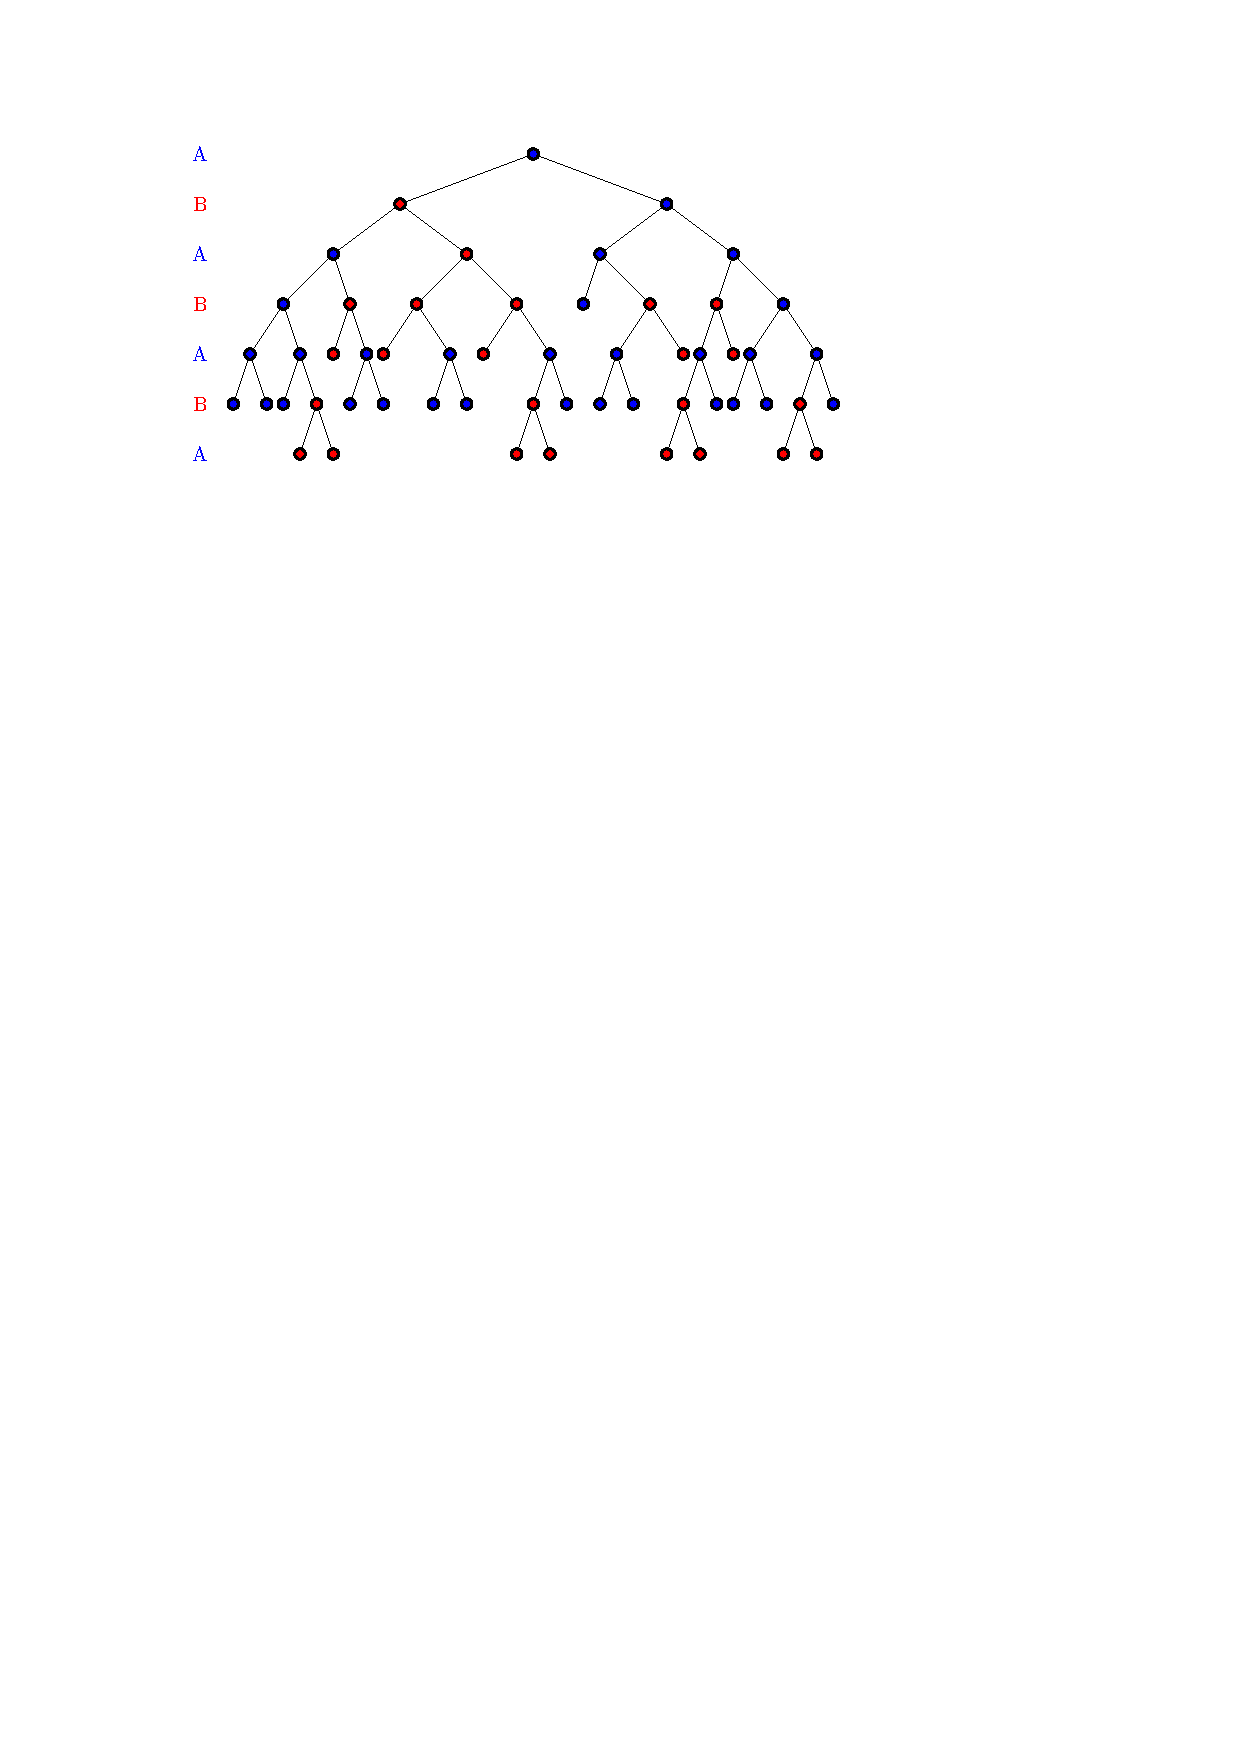
\includegraphics[width=3in]{decisionTree4.pdf}}

  \vspace{1em}

  Continue labeling the entire tree based on when the active player has
  the option to move into their color or not.
\end{frame}

\begin{frame}
  \centerline{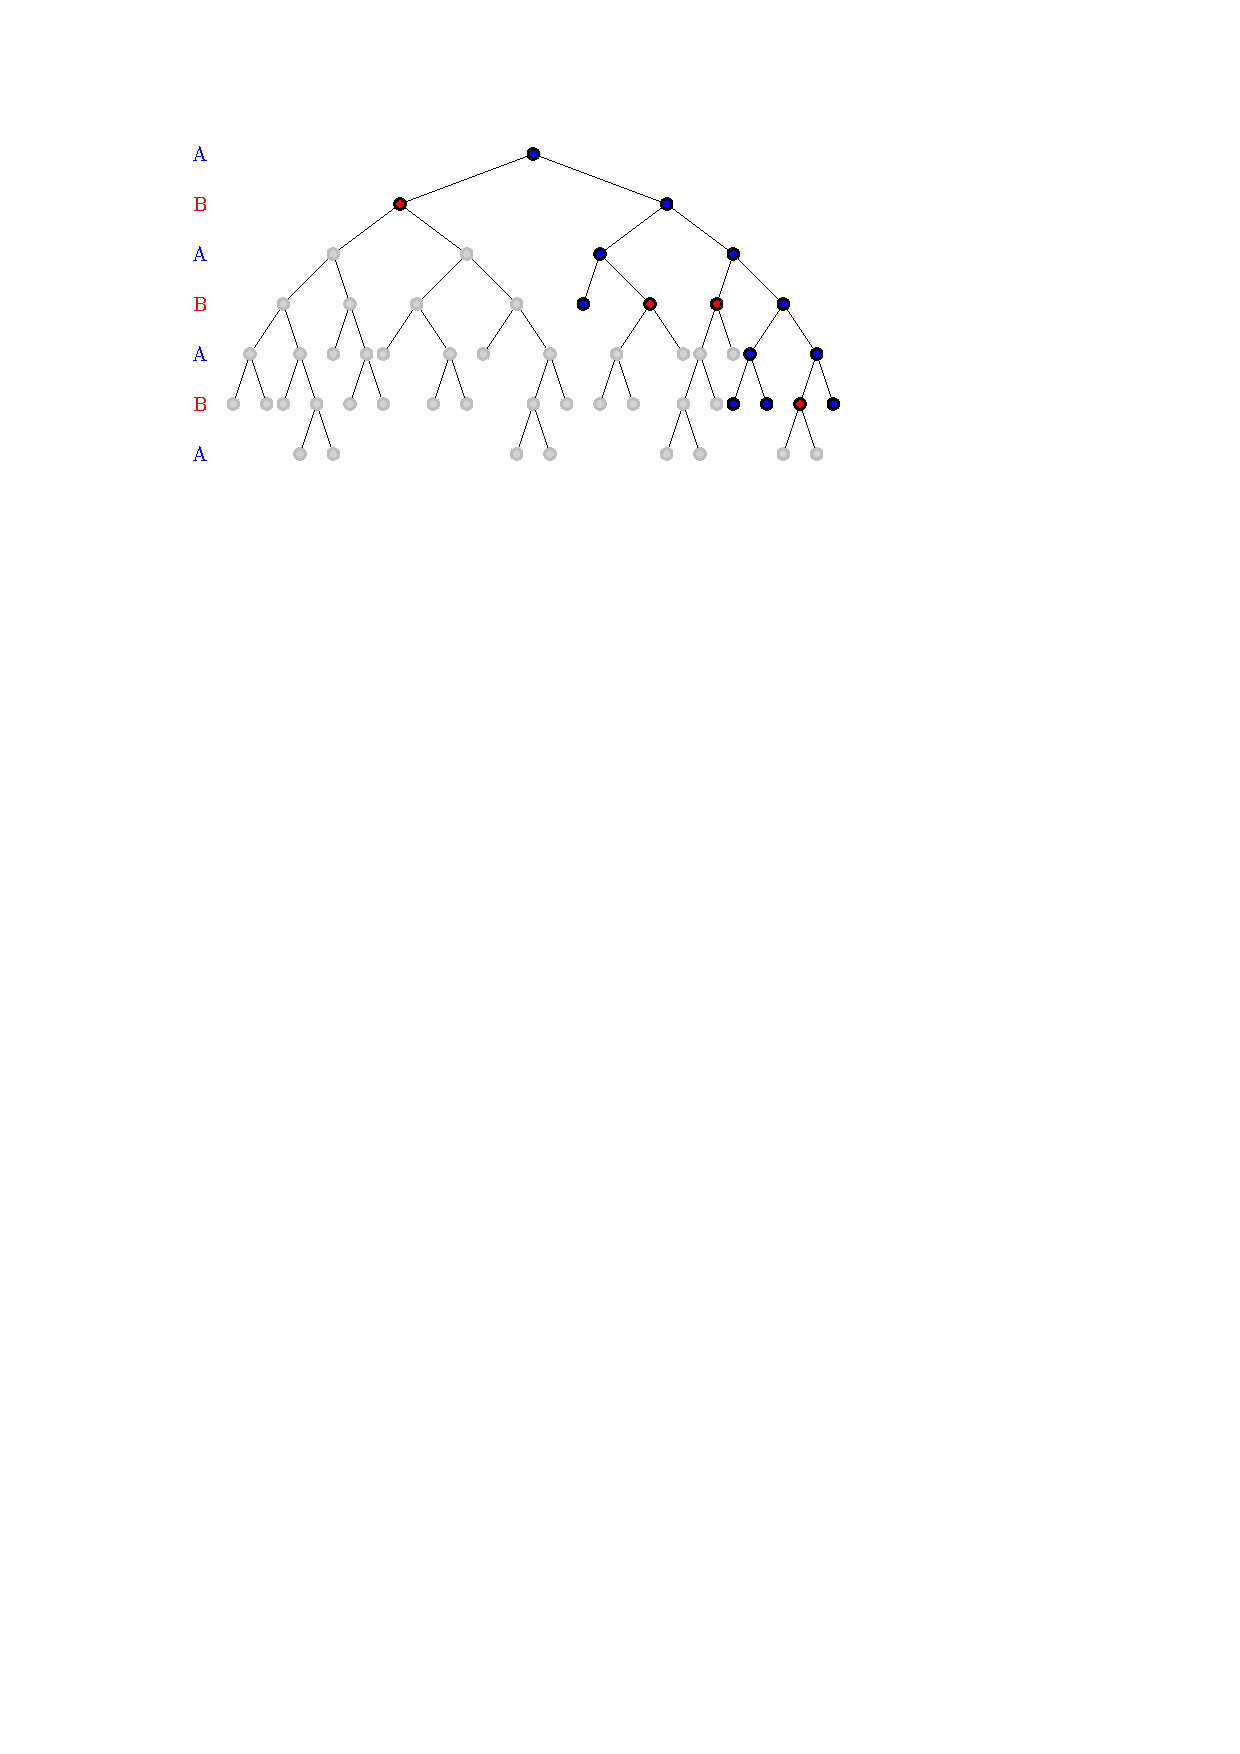
\includegraphics[width=3in]{decisionTree5.pdf}}

  \vspace{1em}

  The color of the top vertex determines which player has the winning strategy.
  This strategy is to always make the decision which moves into the appropriate
  color.
\end{frame}

\subsection{Consequences}

\begin{frame}{So what about chess?}
  Due to Zermelo's theorem, we know that either White or Black has a winning
  strategy in chess: a guaranteed way to prevent losing the game.

  \vpause

  But the problem is, we don't have a way to know exactly what it is! The
  decision tree for chess has millions upon millions of nodes, and our
  computers aren't powerful enough to figure it out (yet). And also, it would
  be so complicated that no human player could memorize it, so there's no
  reason to stop playing now. :-)

  % \vpause

  % (If you're curious, it took $50$ to $200$ desktop computers $18$ years
  % to work together and figure out that both players have a winning strategy
  % in checkers by forcing a draw.)
\end{frame}

\section*{}

\begin{frame}
Questions? Thanks for having me!
\end{frame}


\end{document}


